%%
%% This is file `thesis.tex',
%% generated with the docstrip utility.
%%
%% The original source files were:
%%
%% nudtpaper.dtx  (with options: `thesis')
%%
%% This is a generated file.
%%
%% Copyright (C) 2013 by Liu Benyuan <liubenyuan@gmail.com>
%%
%% This file may be distributed and/or modified under the
%% conditions of the LaTeX Project Public License, either version 1.3a
%% of this license or (at your option) any later version.
%% The latest version of this license is in:
%%
%% http://www.latex-project.org/lppl.txt
%%
%% and version 1.3a or later is part of all distributions of LaTeX
%% version 2004/10/01 or later.
%%
%% To produce the documentation run the original source files ending with `.dtx'
%% through LaTeX.
%%
%% Any Suggestions : LiuBenYuan <liubenyuan@gmail.com>
%% Thanks Xue Ruini <xueruini@gmail.com> for the thuthesis class!
%% Thanks sofoot for the original NUDT paper class!
%%
%1. 规范硕士导言
% \documentclass[master,ttf]{nudtpaper}
%2. 规范博士导言
% \documentclass[doctor,twoside,ttf]{nudtpaper}
%3. 如果使用是Vista
% \documentclass[master,ttf,vista]{nudtpaper}
%4. 建议使用OTF字体获得较好的页面显示效果
%   OTF字体从网上获得,各个系统名称统一,不用加vista选项
%   如果你下载的是最新的(1201)OTF英文字体,建议修改nudtpaper.cls,使用
%   Times New Roman PS Std
% \documentclass[doctor,twoside,otf]{nudtpaper}
%   另外,新版的论文模板提供了方正字体选项FZ,效果也不错哦
% \documentclass[doctor,twoside,fz]{nudtpaper}
%5. 如果想生成盲评,传递anon即可,仍需修改个人成果部分
% \documentclass[master,otf,anon]{nudtpaper}
%
\documentclass[master,otf]{nudtpaper}
\usepackage{mynudt}

\classification{TP391}
\serialno{12060025}
\confidentiality{公开}
\UDC{}
\title{面向规模化无线传感网的数据认证关键技术研究}
\displaytitle{面向规模化无线传感网的数据认证关键技术研究}
\author{蓝宗骁}
\zhdate{\zhtoday}
\entitle{Large-scale Wireless Sensor Network Data Authentication}
\enauthor{Lan Zongxiao}
\endate{\entoday}
\subject{计算机科学与技术}
\ensubject{Computer Science and Technology}
\researchfield{无线网络与移动计算}
\supervisor{夏戈明\quad{}副教授}
\cosupervisor{} % 没有就空着
\ensupervisor{Associate Professor Xia Geming}
\encosupervisor{}
\papertype{工学}
\enpapertype{Engineering}
% 加入makenomenclature命令可用nomencl制作符号列表。




\begin{document}
\graphicspath{{figures/}}
% 制作封面,生成目录,插入摘要,插入符号列表 \\
% 默认符号列表使用denotation.tex,如果要使用nomencl \\
% 需要注释掉denotation,并取消下面两个命令的注释。 \\
% cleardoublepage% \\
% printnomenclature% \\
\maketitle
\frontmatter
\tableofcontents
\listoftables
\listoffigures

\midmatter
% Abstract
\clearpage
\thispagestyle{plain}
\phantomsection
\addcontentsline{toc}{chapter}{Abstract}

\centerline{\zihao{3}\bfseries Abstract}

\linespread{1.4}\zihao{-4}
\bigskip

This thesis explores the relationship between focus structure and pronoun resolution among non-native speakers of English and French. Firstly we reviewed the existing literature on the mechanism of focus effect and pronoun resolution. Then through a self-paced reading test, we find that focus, in the form of cleft structure does not necessarily increase the salience of a informational unit, thus may not in some cases make it a preferred antecedent for pronoun resolution. This result is line with previous researches on this topic. In our experiment, We also find that focused subject in French and focused object in English are processed faster, but focused subjects in both languages leads to longer response time of anaphora. Furthermore, our research also shows that the congruence between anaphora and focus does not make the latter more accessible. In this regard, we argue that the problem of whether there is subject or object preference in English and French is more complicated than the results of current studies.

\bigskip
\noindent\textbf{\zihao{4} Keywords:} 
focus effect, pronoun resolution, self-paced reading, English, French


%\begin{denotation}
\begin{table}[h]%此处最好是h
\caption{国际单位制中具有专门名称的导出单位}
\vspace{0.5em}\centering\wuhao
\begin{tabular}{ccccc}
\toprule[1.5pt]
量的名称&单位名称&单位符号&其它表示实例\\
\midrule[1pt]
频率&赫[兹]&Hz&s-1\\
\bottomrule[1.5pt]
\end{tabular}
\end{table}
\end{denotation}


%书写正文,可以根据需要增添章节; 正文还包括致谢,参考文献与成果
\mainmatter
\chapter{绪论}
本章介绍了无线传感网的结构及其应用领域。分析规模化无线传感网的特点,对规模化传感网数据认证的需求和面临的挑战进行了分析。概述了本文的研究内容,并对文章的组织结构予以说明。
\section{本文研究背景和意义}
无线传感器网络(Wireless Sensor Networks,无线传感网)是一种特殊组织结构的移动自组网\upcite{c:sensor},在环境监测、工业控制、资源监控、智能家居、医疗保健和军事等各种领域都有广泛应用,有非常重要的地位和作用。
随着无线传感网技术的不断发展,很多应用进入了日常生活中,物联网技术也将成为未来发展的重要方向。
无线传感网的各种技术发展紧跟具体的应用需求,随着各种应用场景需要的安全性越来越高,安全问题也成为了阻碍无线传感网大规模发展的一个制约。

大范围监测在环境监测和军事侦察等诸多关系国家社会重大安全的领域都具有重要的地位和作用。在环境监测领域,往往面临范围野外受限甚至恶劣条件,在海洋等资源监测领域,水声通信等基础技术还不是很完善, 在军事侦察对抗领域更是要应对破坏攻击情况,传统的大范围实时监测机制和系统都难以得到有效部署,使用无线传感技术成为了最好的解决方案。规模化无线传感网因此应运而生,而且为满足大范围监测的需要,无线传感网的规模越来越大。

规模化无线传感网面临的安全威胁更多,攻击的影响更大,而且由于传感器节点的特点,传统的安全机制和协议无法直接适用于无线传感网,使得安全问题更加凸显。因此针对规模化无线传感网安全机制的研究成为了热门研究方向。

\subsection{无线传感网概述}
\subsubsection{无线传感网结构}
无线传感器节点被部署在目标监测区域,大量的传感器节点通过无线广播的方式,以一定的算法自组织成为一个多跳的无线网络。如图~\ref{fig:cluster}所示,是一个典型无线传感网的结构\upcite{c:cluster},由三部分组成:监测区域的传感器节点、与外部网络连接的网关或基站、远程数据中心。在监测区域的传感器节点一般通过算法组成若干的簇,每个簇通过簇头节点与其他簇或者基站通信,这样的方案节约了节点的能量。簇内节点收集到监测数据以后通过簇头节点的整合,形成报文通过一定的路径发送给基站,基站进一步通过外部网络设备,如互联网、卫星等将监测数据传输到远程数据中心。

\begin{figure}[htbp]
  \centering
  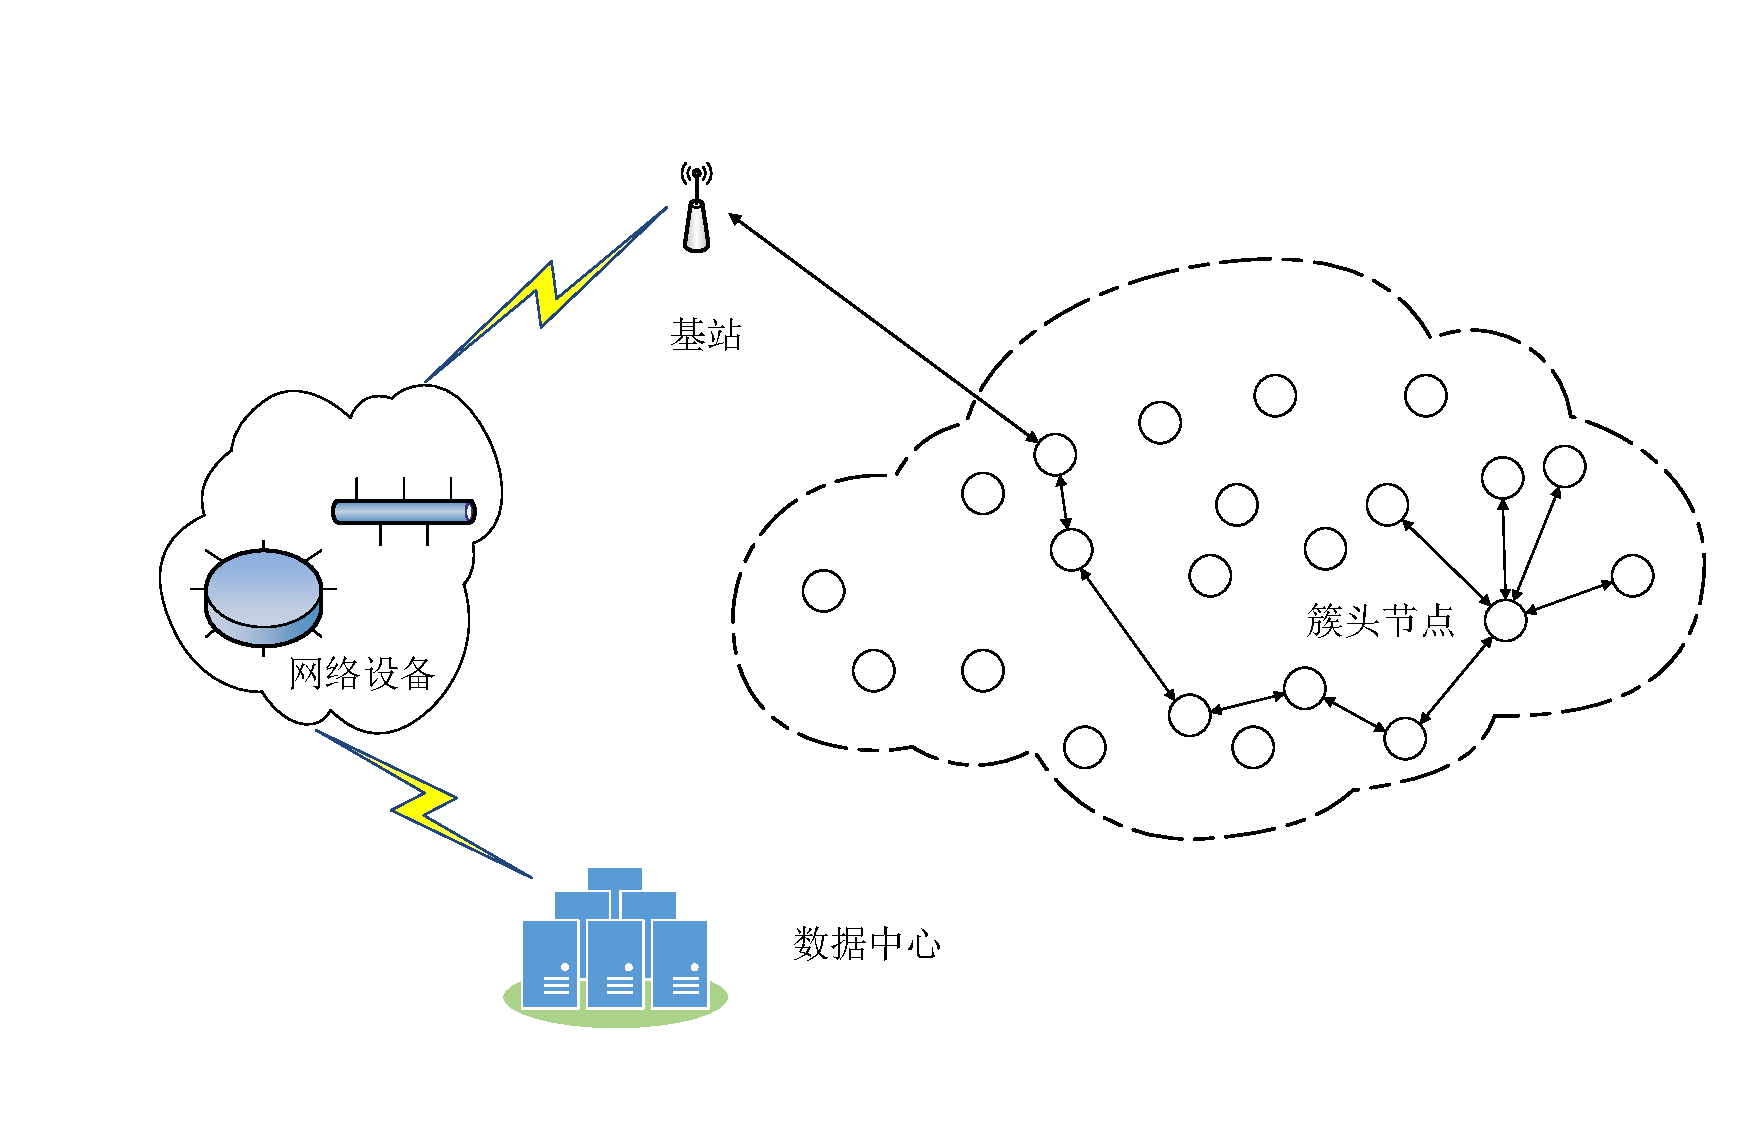
\includegraphics[width=5in]{cluster}
  \caption{无线传感网系统结构}
  \label{fig:cluster}
\end{figure}


无线传感网中,基站的计算和存储能力都比较强,
基站的功能可以是一个数据处理中心,向网络广播控制信息,从监测区域获取数据。
也可以是一个网络网关,负责数据向远程数据中心的传输。

\subsubsection{无线传感器节点结构}
传感器节点是无线传感网的基本组成单元,负责数据采集、发送等基本功能。
无线传感器节点一般仅具有很小的存储空间,较弱的计算能力,因此单个节点无法完成复杂的感知任务,需要大量的节点协同工作。

随着电子技术的发展,无线传感器节点的性能也有了很大的提升,如Crossbow公司研发的TelosB,CPU频率为8MHz,有10KB的RAM,使用2.4GHz无线电,能达到250Kbps数据传输,使用两节AAA电池(5号电池)供电。国产传感器节点典型的有美新的MEMSIC无线模块,工作频率可选433 MHz、868-915MHz或2.4GHz,拥有5年电池寿命,支持10-100米的发射范围,拥有19.2kbps-240kbps的数据传输速率。

\begin{figure}[htbp]
  \centering
  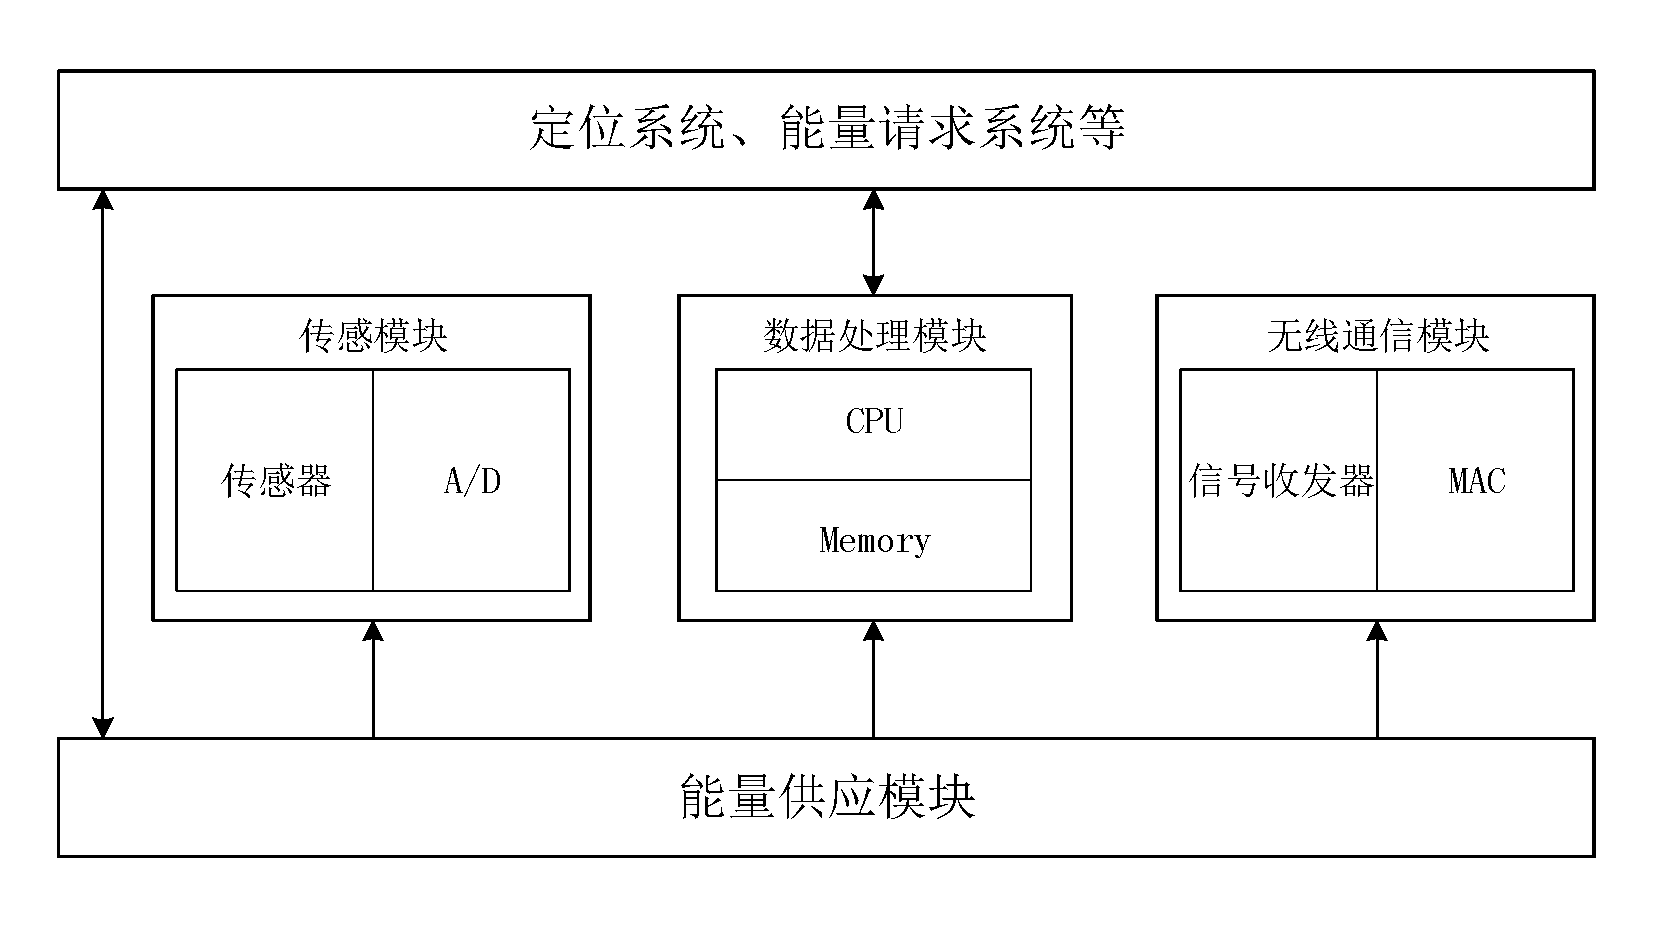
\includegraphics[width=5in]{node}
  \caption{无线传感网节点结构}
  \label{fig:node}
\end{figure}

这些传感器节点的设计原理基本相同,主要包括4个模块:传感模块、数据处理模块、无线通信模块和能量供应模块。
如图~\ref{fig:node}所示,是一个典型的无线传感器节点的结构图。传感模块主要负责从感知区域通过传感器获取数据,并将数据转化为适合进行网络传输的数字信号;数据处理模块主要包括处理和存储功能,负责控制传感器节点的运行,对传感模块获取的数据进行处理和存储,数据报文的整合与认证都是由数据处理模块完成,一般该模块需要嵌入式系统的支持,如UC Berkeley的开源嵌入式系统TinyOS\upcite{c:tinyos}等;无线通信模块负责与其他传感器节点或基站之间的通信,传感器节点一般使用内置天线进行数据收发;能量供应模块负责给其他模块供应能量,大部分传感器节点使用微型电池作为电源,因此能量非常有限。传感器节点中还包括一些负责定位、同步等功能的部件。

\subsubsection{无线传感网协议结构}

\begin{figure}[htbp]
  \centering
  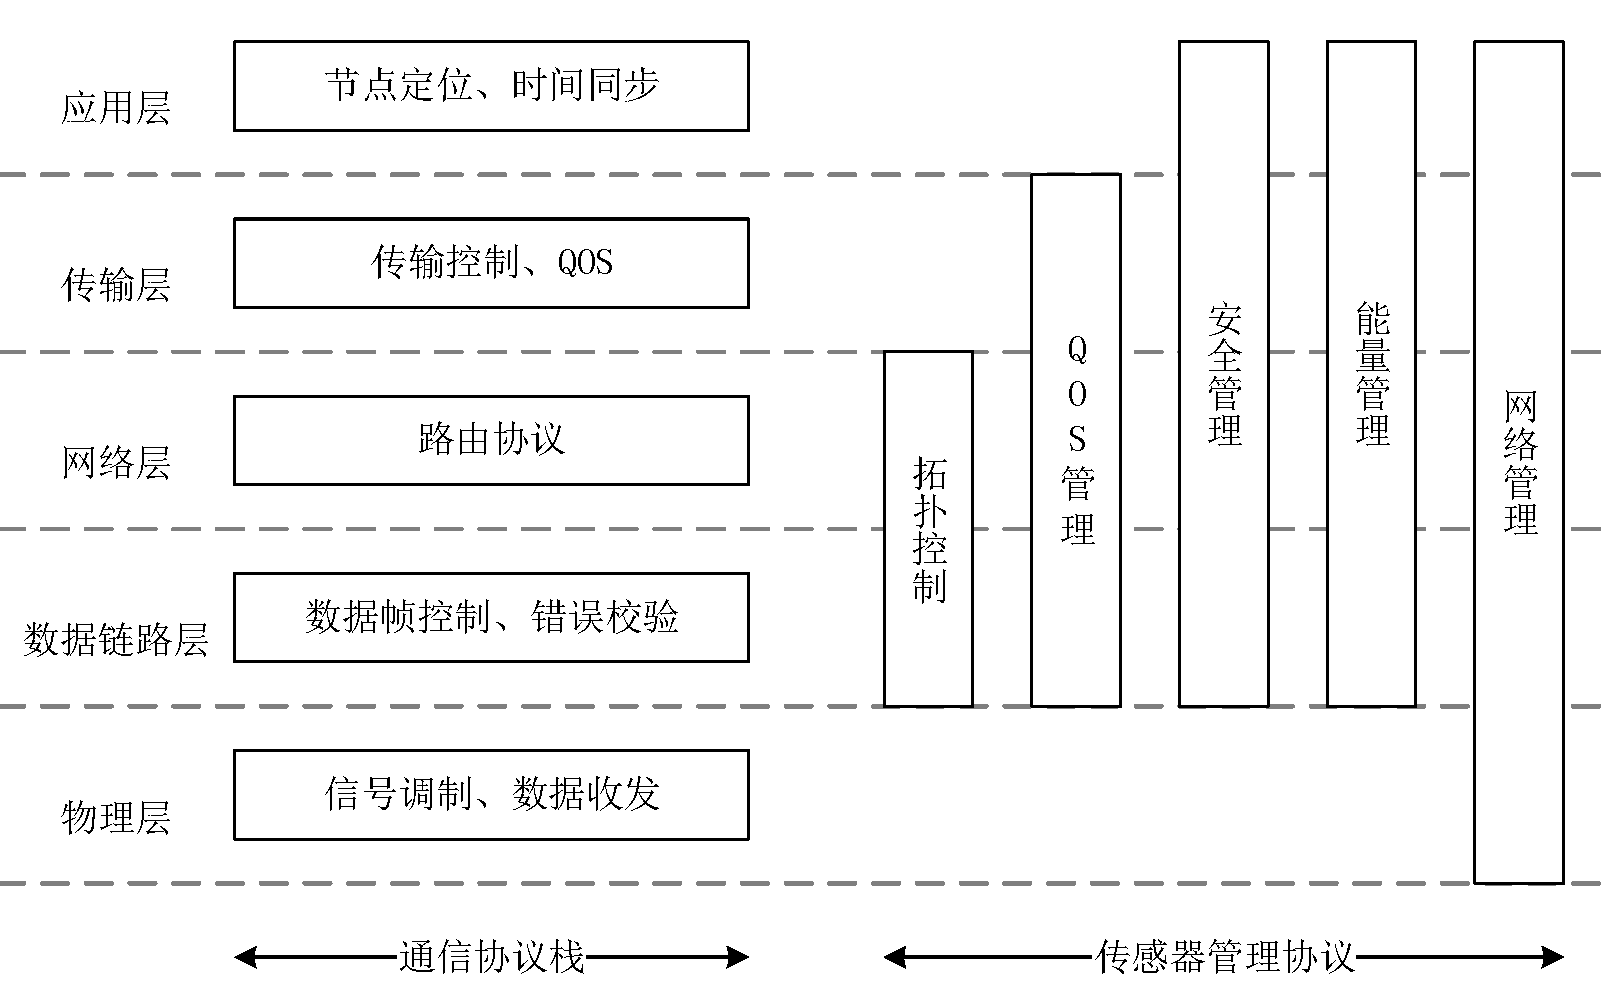
\includegraphics[width=5in]{construction}
  \caption{无线传感网协议结构}
  \label{fig:construction}
\end{figure}
无线传感网的通信协议栈和相关网络管理技术是当前的主要研究内容,协议结构如图~\ref{fig:construction}所示。
因为无线传感网是面向特定需求的网络,因此针对不同的部署环境,不同的网络部署结构,要对通信协议栈进行优化,使能量消耗、抗节点损耗、抗攻击能力等适应传感网的应用需求。

类似于OSI网络模型,无线传感网的通信协议栈由物理层、数据链路层、网络层、传输层、应用层组成:

物理层:物理层是通信协议栈的最底层,主要功能是将数据调制成适合传输的数字信号,通过无线电、红外灯无线介质完成传感器节点的数据收发。

数据链路层:数据链路层负责装配数据帧,对数据帧进行MAC校验,进行差错控制,向网络层提供透明可靠的数据传输服务。

网络层:主要负责无线传感网中的路由功能,将数据通过有效路径传送到目标节点,向传输层提供端对端的数据传输服务。

传输层:传输层负责数据报文的传送和控制,为应用层提供可靠的传输服务,对网络进行流量控制,进行服务质量控制(QOS)。

应用层:直接为应用提供服务,提供相应的应用协议和服务接口。

传感网管理协议提供了拓扑管理、QOS管理、安全管理、能量管理和网络管理等功能,实现对无线传感网以及各个节点的监控和管理。
\subsubsection{无线传感网的应用前景}
分布式传感网在军事中的应用是无线传感网的雏形,随着电子技术的不断发展,传感器节点的性能不断提升,无线传感网各种协议的完善和发展,使无线传感网在环境监测、军事侦察、智能家居、智能公路等各个领域得到了大量的应用,其应用前景十分广泛。

\begin{compactitem}
  \item 环境监测:无线传感网能完成大范围监测的任务,在自然数据采集中发挥重要作用,尤其是海洋监测传感网和内陆水文传感网等应用领域。如Li 等人将无线传感网部署在水产养殖水域,对水环境数据进行检测\upcite{c:water}。
  \item 军事侦察:由于无线传感网具有自组网、部署简单、容许节点失效等特点,适合部署在危险的敌对区域,完成军事侦察、战场环境监测等任务,因而在军事领域有很大应用前景,是现代化电子战的重要战略武器。如美国海军将开发的自主分布式DADS(Deployable Autonomous Distributed System)用于沿海广大海域的警戒、反潜和反水雷\upcite{c:DADS}。
  \item 智能家居:智能家居是通过无线传感器将房间中的各种家电等设备连接起来,实现家居环境的监测以及远程控制,构建出智能的居住环境\upcite{c:homes}。
  \item 智能公路:通过部署在公路上的无线传感器节点以及车载传感器节点,共同组成智能公路传感网络,对交通状况实现自动监测,引导车流等,实现自动化的公路交通管理。
\end{compactitem}



\subsection{规模化无线传感网数据认证}
\subsubsection{规模化无线传感网的特点}
规模化无线传感网是为满足大范围监测的需要而产生的,如国内著名的绿野千传项目,在浙江省天目山建立的大规林业监测传感网,部署的自组织传感网节点超过2000个,网络中传输路径跳数超过 20 跳
\upcite{c:lvye}。
规模化无线传感网具有如下的特点:
\begin{enumerate}\setlength{\itemsep}{-\itemsep}
  \item 节点数量大,覆盖面积广,节点失效较为频繁,网络拓扑结构相对不稳定。
  \item 一般部署于恶劣区域,甚至是敌对攻击区域,恶意攻击的频度增加。
  \item 节点的计算和存储能力更为受限,网络的能量较为敏感,对机制的轻量化要求更突出。
\end{enumerate}

\subsubsection{规模化无线传感网的数据认证需求}
无线传感网中的认证包括身份认证和数据认证。身份认证是对网络中节点的合法身份的一种判定机制,是数据认证的基础。无线传感网数据认证主要包括两个方面:
\begin{compactitem}
  \item 数据来源合法性,主要以身份认证为基础,通过数据报文中的认证机制判定数据报文的来源的合法性。
  \item 数据完整性,通过数据认证的机制,确保节点收到的数据报文没有被非法进行篡改。
\end{compactitem}

在环境监测等领域,规模化传感网每天都会产生海量的感知数据。在军事侦察领域,随着侦察区域的扩大,侦察精度的提高,传感网感知的数据量飞速增长。尤其在实时监测场景,数据量大、传输实时性要求高,无线传感器节点的性能限制使得规模化传感网实现可靠传输具有非常的难度,合适的数据认证机制可以为其提供有力支持。在无线传感网中数据泄露、错误数据甚至虚假数据会对网络的安全造成重大影响。尤其在重要战略场景或军事场景,还要考虑破坏攻击的可能,因此数据认证更为安全攸关。
\subsubsection{规模化无线传感网数据认证面临的挑战}

复杂环境下数据高安全性要求对数据认证提出的挑战。实时监测传感网通常部署环境恶劣,而且缺乏基础设施的建设,由于自然环境和主动攻击等对节点的破坏,使节点的失效率很高,网络拓扑结构动态变化,数据传输质量不够稳定,而且存在突发大故障潜因,需要在容灾抗毁前提下进行数据认证,确保传输的安全性。

端对端传输为数据认证提出的挑战。完全依靠广播等数据传输机制,在规模化无线传感网中,传输效率过低,消耗的节点能量和通信资源过大,而且容易受到泛洪攻击的影响。有效利用规模化传感网中端对端数据传输,能够有效的保证传输效率。在端对端传输中,由于多跳传输的原因,当路径中出现妥协节点时,整条路径容易被攻破,从而造成数据传输被攻击,因而在多路径端对端的数据传输中,有效利用数据认证机制加强路径上的安全保障是安全传输的关键。

轻量级认证机制及其实现技术为数据认证提出的挑战。规模化无线传感网传输的数据量大,要求处理快捷。在节点资源能力受限,通信能耗受限的前提下,需要计算、存储、通信都轻量级的水平,保障网络安全、传输可靠性、高效性和数据可信,具有很大难度。传统的的认证机制使用的密码算法复杂度未达到轻量级,不适合规模化传感网网络资源受限的特点,我们需要设计适合实时性较高的规模无线传感网达到轻量级算法。

攻击对抗对数据认证提出的挑战。无线传感网一般部署在恶劣环境中,而且具有自组网络的多跳性、无中心性和自组织性等特征,致使其通信协议栈的各个层级都容易遭受到各种形式的攻击,我们需要设计能够适应有限节点能量,有限计算能力的数据认证算法,对抗各种攻击,保证无线传感网传输数据的来源合法性和完整性。

\section{本文研究内容}
本文根据规模化无线传感网的安全需求以及其特点,针对其数据认证关键技术展开研究,使用多节点联合的技术思路研究数据认证模型和机制,并设计实现了关键算法。
主要工作如下:

\begin{enumerate}\setlength{\itemsep}{-\itemsep}
  \item 提出了多跳长路径上多节点联合数据认证的模型,设计了多跳长路径上多节点联合数据认证协议,并设计了路径上节点关系的维护算法,对协议的安全性能进行了分析评价。
  \item 针对多跳长路径上多写点联合数据认证协议的不足,对算法进行了优化,提出了多路径抗节点失效机制和动态步长多节点联合数据认证机制,并对优化方案的安全性能进行了分析评价。
  \item 围绕多跳长路径多节点联合数据认证机制的需求,对密钥分配方案进行了深入研究,提出了基于单向hash链的密钥分配方案,并对认证中的MAC进行了研究,提出了适应数据认证机制需求的MAC码。
\end{enumerate}


\section{本文组织结构}
本文一共分为七章。

第一章\quad 绪论,介绍了课题的选题背景,描述了无线传感网的特点,介绍了无线传感网的相关安全技术,列出了本文的主要研究内容和本文组织结构。

第二章\quad 相关研究概述,本章首先对无线传感网的安全技术进行了概述,然后重点对数据认证和密钥分配两种安全技术进行了论述。

第三章\quad 多跳长路径上多节点联合数据认证,本章提出了无线传感网中多跳长路径多节点联合的数据认证模型,及其设计目标。
重点介绍了关键算法与协议的设计实现,对多节点联合数据认证机制的安全性能进行了分析评价。

第四章\quad 数据认证方案优化,本章针对多跳长路径上多节点联合数据认证进行了优化,提出了多路径抗节点失效和动态步长多节点联合数据认证两个优化方案,并对它们的安全性能进行了分析评价。

第五章\quad 密钥分配与MAC设计,本章对多节点联合数据认证中的密钥分配方案以及使用的MAC的设计进行了介绍,提出了基于单向hash链的密钥分配方案,以及适应多节点联合数据认证的MAC码。

第六章\quad 仿真实验与结果分析,本章在仿真平台上对多跳长路径多节点联合数据认证机制,以及其优化方案进行了仿真实验,对它们的安全性能结果进行了评价。

第七章\quad 总结与展望,本章对全文的工作做了总结,指出了数据认证机制现阶段的不足以及未来研究中需要研究及完善的地方。


\chapter{中华人民共和国}
\label{cha:china}

\section{图的例子}
\label{sec:other}

在第~\ref{cha:intro} 章中我们学习了贝叶斯公式~(\ref{equ:chap1:bayes}),这里我们复
习一下:
\begin{equation}
\label{equ:chap2:bayes}
p(y|\mathbf{x}) = \frac{p(\mathbf{x},y)}{p(\mathbf{x})}=
\frac{p(\mathbf{x}|y)p(y)}{p(\mathbf{x})}
\end{equation}

\subsection{绘图}
\label{sec:draw}

本模板不再预先装载任何绘图包(如 \textsf{pstricks,pgf} 等),完全由你自己来决定。
个人觉得 \textsf{pgf} 不错,不依赖于 Postscript。此外还有很多针对 \LaTeX{} 的
 GUI 作图工具,如 XFig(jFig), WinFig, Tpx, Ipe, Dia, Inkscape, LaTeXPiX,
jPicEdt, jaxdraw 等等。

\subsection{插图}
\label{sec:graphs}
关于子图形的使用细节请参看 \textsf{subcaption} 的说明文档。

\subsection{一个图形}
\label{sec:onefig}
一般图形都是处在浮动环境中。之所以称为浮动是指最终排版效果图形的位置不一定与源文
件中的位置对应\footnote{This is not a bug, but a feature of
\LaTeX!},这也是刚使 用 \LaTeX{}
同学可能遇到的问题。如果要强制固定浮动图形的位置,请使用
\textsf{float} 宏包, 它提供了 \texttt{[H]}
参数,比如图~\ref{fig:heythere}。
\begin{figure}[H] % use float package if you want it here
  \centering
  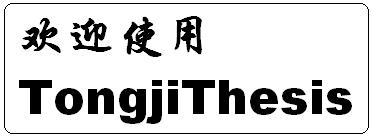
\includegraphics[height=2cm]{hello.jpg}
  \caption{插个图插个图}
  \label{fig:heythere}
\end{figure}

大学之道,在明明德,在亲民,在止于至善。知止而后有定;定而后能静;静而后能安;安
而后能虑;虑而后能得。物有本末,事有终始。知所先后,则近道矣。古之欲明明德于天
下者,先治其国;欲治其国者,先齐其家;欲齐其家者,先修其身;欲修其身者,先正其心;
欲正其心者,先诚其意;欲诚其意者,先致其知;致知在格物。物格而后知至;知至而后
意诚;意诚而后心正;心正而后身 修;身修而后家齐;家齐而后国治;国治而后天下
平。自天子以至于庶人,壹是皆以修身为本。其本乱而未治者 否矣。其所厚者薄,而其所
薄者厚,未之有也!

\hfill \pozhehao《大学》


\subsection{简单子图}
\label{sec:multifig}

如果多个图形相互独立,并不共用一个图形计数器,那么用 \verb|minipage| 或者
\verb|parbox| 就可以。否则,请参看图~\ref{fig:big1},它包含两个小图,分别是图~\ref{fig:subfig1}
和图~\ref{fig:subfig2}。推荐使用 \verb|\subcaption|,不要再用\verb|\subfloat|,\verb|\subfigure| 和 \verb|\subtable|了。
\begin{figure} %[h]
  \centering%
  \subcaptionbox{第一个小图形\label{fig:subfig1}}{%    
    
\includegraphics[height=2cm]{tongji-fig-logo.png}}\hspace{4em}%
  \subcaptionbox{第二个小图形。如果标题很长的话,它会自动换行,这个 caption 就是这样的例子\label{fig:subfig2}}{%    
    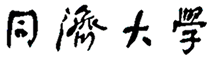
\includegraphics[height=2cm]{tongji-text-logo.png}}
  \caption{包含子图形的大图形}
  \label{fig:big1}
\end{figure}

古之学者必有师。师者,所以传道受业解惑也。人非生而知之者,孰能无惑?惑而不从师,
其为惑也,终不解矣。生乎吾前,其闻道也固先乎吾,吾从而师之;生乎吾後,其闻道也亦
先乎吾,吾从而师之。吾师道也,夫庸知其年之先後生於吾乎!是故无贵无贱无长无少,道
之所存,师之所存也。

嗟乎!师道之不传也久矣,欲人之无惑也难矣。古之圣人,其出人也远矣,犹且从师而问焉;
今之众人,其下圣人也亦远矣,而耻学於师。是故圣益圣,愚益愚。圣人之所以为圣,愚
人之所以为愚,其皆出於此乎?爱其子,择师而教之,於其身也,则耻师焉,惑焉。彼童子
之师,授之书而习其句读者,非吾所谓传其道、解其惑者也。句读之不知,惑之不解,或师
焉,或不焉,小学而大遗,吾未见其明也。巫医、乐师、百工之人不耻相师,  士大夫之族
曰“师”曰“弟子”之云者,则群聚而笑之。问之,则曰:彼与彼年相若也,道相似也,位
卑则足羞,官盛则近谀。呜呼!师道之不复,可知矣。巫医、乐师、百工之人。吾子不齿,
今其智乃反不能及,其可怪也欤!圣人无常师。孔子师郯子、苌子、师襄、老聃。郯子之徒,
其贤不及孔子。孔子曰:“三人行,必有我师。”是故弟子不必不如师,师不必贤於弟子。
闻道有先後,术业有专攻,如是而已。

\subsection{复杂子图要注意遮挡}
使用子图的方法如图~\ref{fig:chap2:zitu}所示,使用\texttt{subcaptionbox}环境设置每一个子图,注意\texttt{subcaptionbox}其后需要有括号,以及子图换行时需要使用\texttt{vskip},以免下一排子图会对上一排子图的图名造成遮挡。
\begin{figure}[htbp]
\centering
  \subcaptionbox{第一个小图形}{\label{fig:chap1:zitu:a}
  
\includegraphics[width=5cm]{tongji-fig-logo}\hskip2cm}
  \subcaptionbox{第二个小图形}{\label{fig:chap1:zitu:b}
  
\includegraphics[width=5cm]{tongji-fig-logo}}
\vskip0.5cm
  \subcaptionbox{第三个小图形}{\label{fig:chap1:zitu:c}
  
\includegraphics[width=5cm]{tongji-fig-logo}\hskip2cm}
  \subcaptionbox{第四个小图形}{\label{fig:chap1:zitu:d}
  
\includegraphics[width=5cm]{tongji-fig-logo}}
\caption{多子图用\texttt{subcaptionbox}}\label{fig:chap2:zitu}
\end{figure}


\subsection{多个图形独立}
如果要把编号的两个图形并排,那么小页就非常有用了,如图~\ref{fig:parallel2}:
\begin{figure}
\begin{minipage}{0.48\textwidth}
  \centering
  
\includegraphics[height=2cm]{tongji-whole-logo.png}
  \caption{并排第一个图}
  \label{fig:parallel1}
\end{minipage}\hfill
\begin{minipage}{0.48\textwidth}
  \centering
  
\includegraphics[height=2cm]{tongji-whole-logo.png}
  \caption{并排第二个图}
  \label{fig:parallel2}
\end{minipage}
\end{figure}


李氏子蟠,年十七,好古文、六艺,经传皆通习之,不拘於时,学於余。余嘉其能行古
道,作师说以贻之。

\hfill \pozhehao 韩愈(唐)


\subsection{插图大原则}
同志们,如果遇到问题一定要会搜索,要么看别人的问答,要么看宏包的文档,希望你不要成为重度伸手党。
一点微小的工作,谢谢大家。

\section{插入pdf格式图片的问题}
\label{sec:problem}
在\LaTeX{}中插入高清图片一般有两种方式:1)插入~eps~矢量图,2)插入~pdf~格式图片。在模板测试过程中遇到一个插入
~pdf~格式图片的问题。

问题描述

插入~pdf~格式的图,有时采用~XeLaTeX~编译后,插图被翻转~90~度。有时却不会出现该问题。问题图片如图~\ref{rotatedBode}~所示。
\begin{figure}[H] 
  \centering
  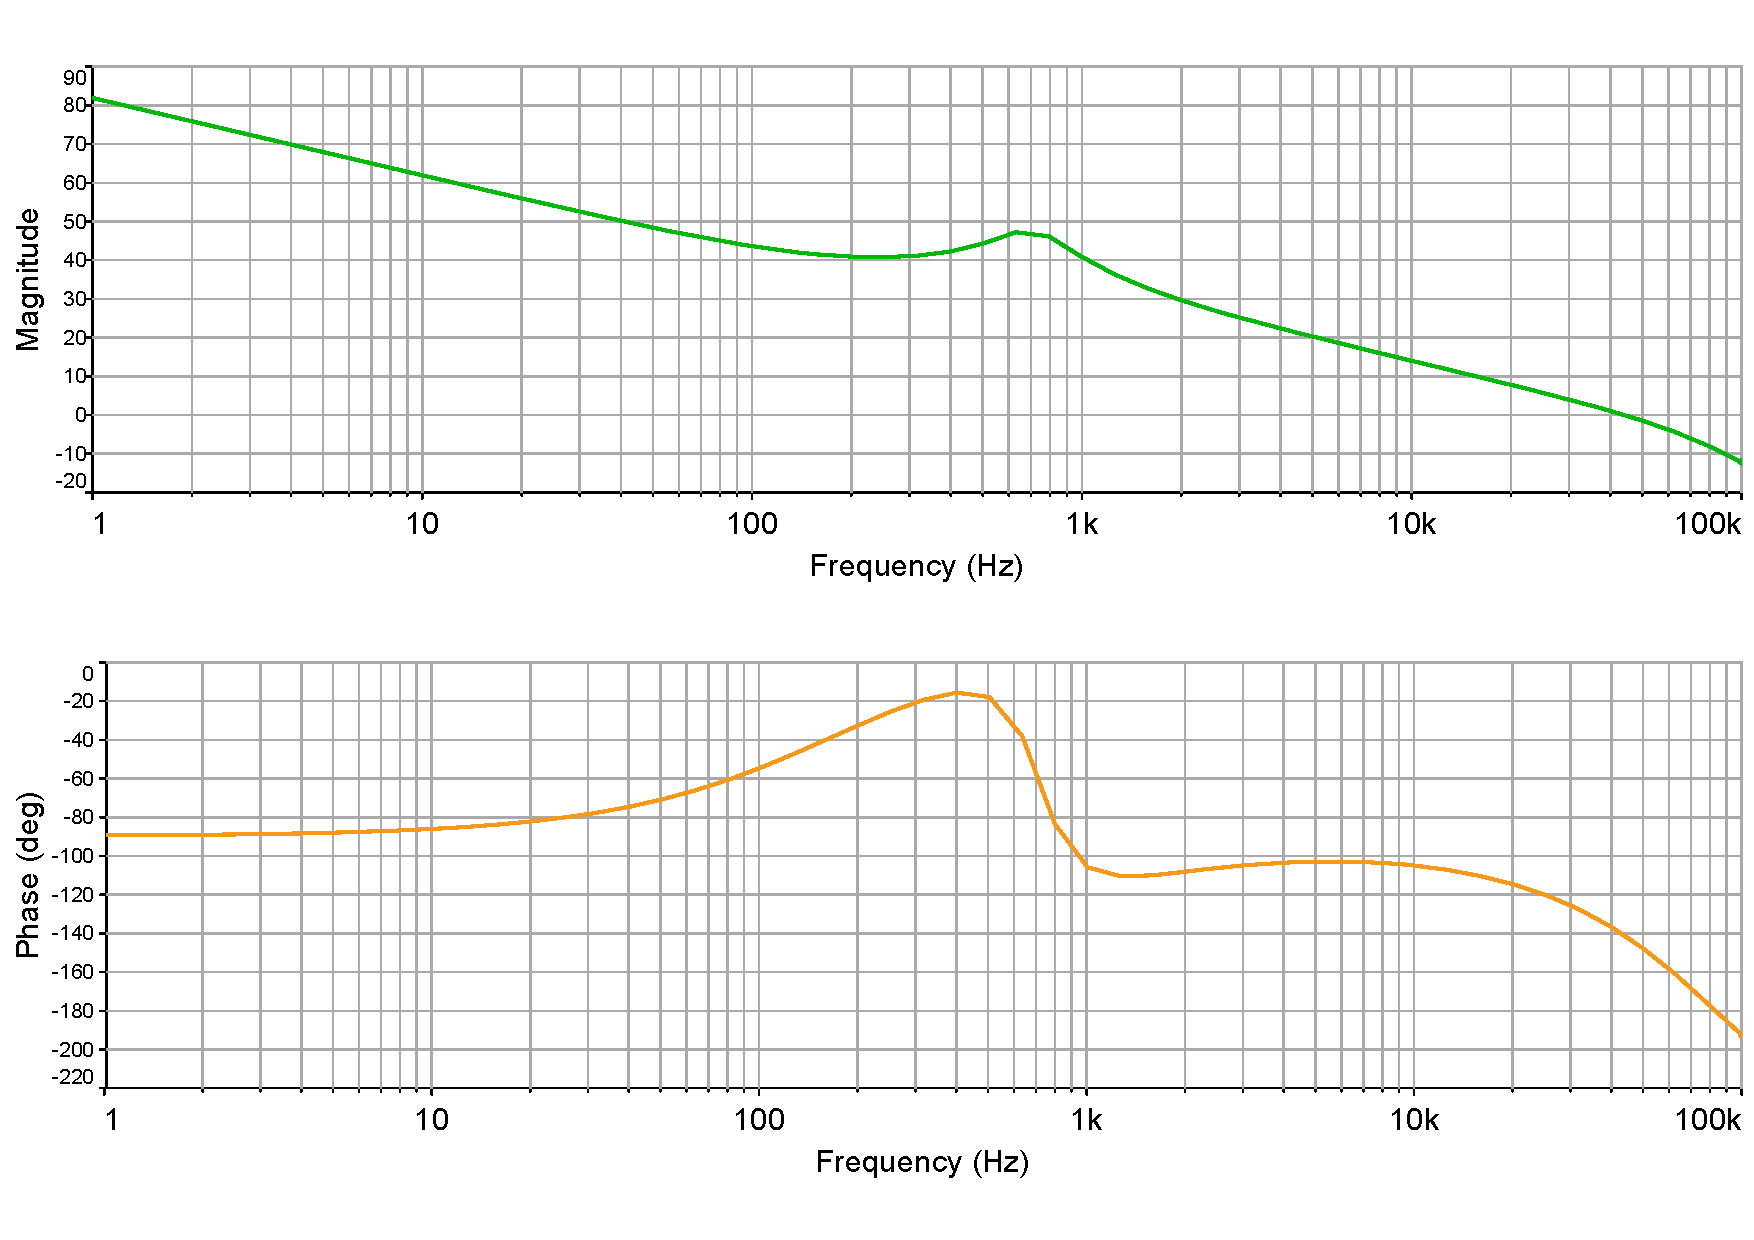
\includegraphics[width=12cm]{BodeGraph.pdf}
  \caption{被自动翻转的bode图}
  \label{rotatedBode}
\end{figure}

问题原因

同一幅图片,XeLaTeX~编译出现图片翻转,而~pdfLaTeX~编译,输出正常。
原因可能是出现在~XeLaTeX~编译过程中会将有些~pdf~文件自身多余的旋转命令编译出来。

问题解决方法

第一种方法(抄自刘海洋大牛的方案):
使用命令\\ \texttt{pdfcrop foo.pdf foo-new.pdf},当然,新文件名可以和旧文件名相同。 这个方法的好处就是 pdfcrop 是texlive自带的,我装的是texlive2017,因此自带了。

第二种方法:采用GhostScript软件消除多余的旋转命令。
\begin{enumerate}
    \item 下载安装~GhostScript~软件,官网为\url{https://www.ghostscript.com/download/gsdnld.html/}
        
    \item 将安装后的bin文件夹地址加入用户环境变量,在我电脑上为~\verb|D:|\verb|\Program Files|\verb|\gs|\verb|\gs9.22|\verb|\bin|
	
    \item cmd~命令行进入想转换图片所在文件夹,执行命令\\gswin32c -sDEVICE=pdfwrite -o newname.pdf  previousname.pdf
              得到一个去除多余旋转命令的~newname.pdf~文件。

    \item 在\LaTeX{}中插入该~pdf~文件,XeLaTeX~编译。
\end{enumerate}

处理之后的图片如图~\ref{Bode}~所示。
\begin{figure}[H] 
  \centering
  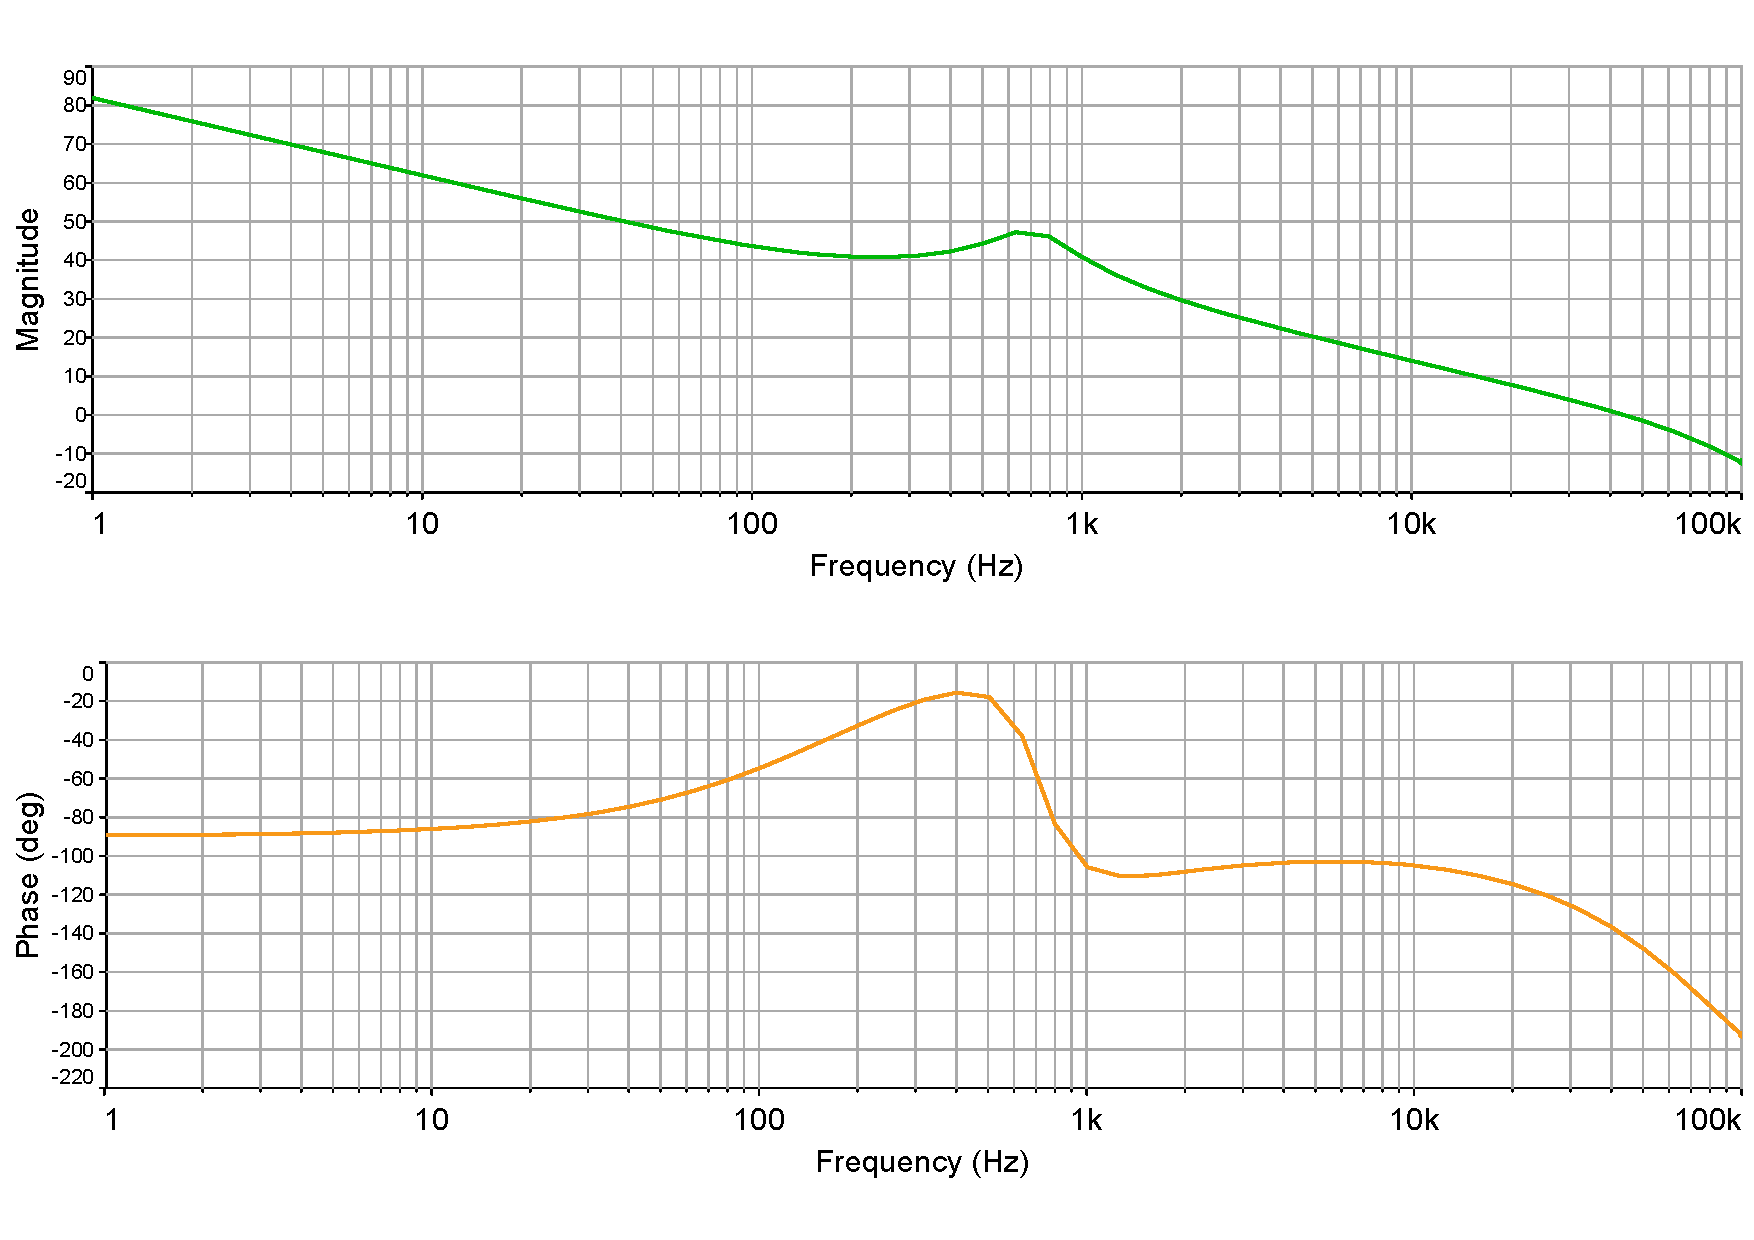
\includegraphics[width=12cm]{Bode.pdf}
  \caption{处理后的bode图}
  \label{Bode}
\end{figure}






\section{网络模型结构}
\subsection*{网络模型结构}
\frame{
  \frametitle{网络整体结构}
	\begin{figure}[h]
		\centering
		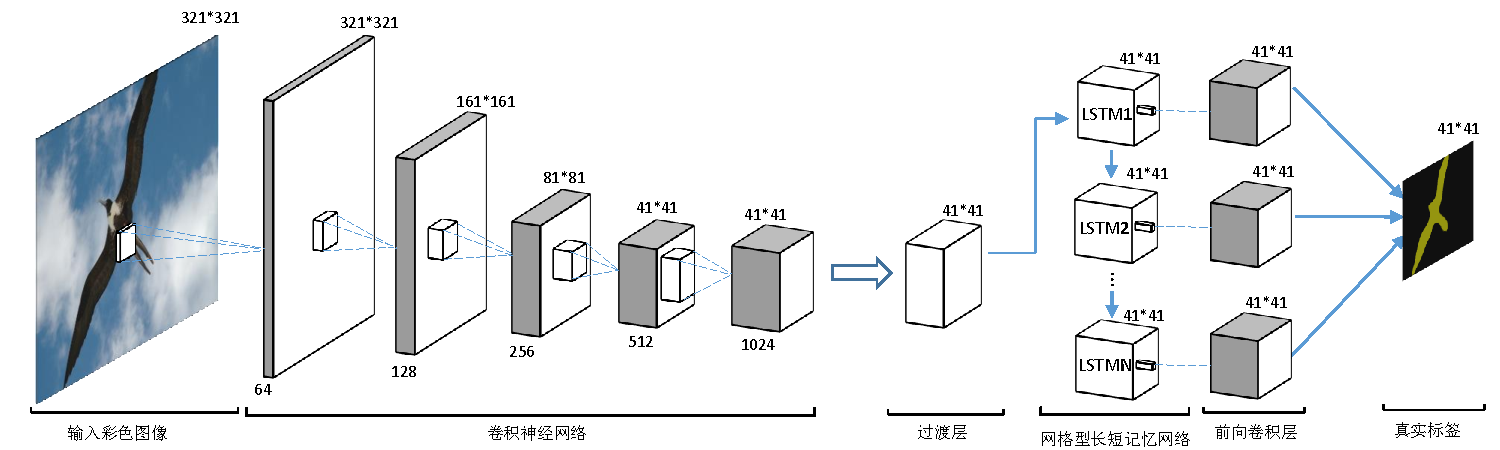
\includegraphics[width=0.9\textwidth,height=0.28\textwidth]{image/illustration/networkstructure.pdf}
		\caption{网络整体结构图}
		\label{fig:networkstructure}
	\end{figure}
	\vspace{-1em}
	\small
	\begin{block}{}
	\begin{itemize}
		\item  四个组成部分:\textbf{卷积网络部分},过渡层,\textbf{网格型长短记忆网络部分},前向卷积层
		\item 核心思想:在卷积网络后堆叠多层网格型长短记忆层
	\end{itemize}
	\end{block}
}
\frame{
	\frametitle{卷积网络部分}
	\vspace{-1em}
	\footnotesize
	\begin{block}{}
	\begin{itemize}
		\item 基于$VGG_{16}$模型\footnote{Simonyan \& Zissermanet, Very deep Convolutional Networks For Large-scale Image Recognition, ICLR 2015}, 含有16层卷积层
		\item 使用了“孔算法”,在不损失精度的情况下将模型参数减少了 6.5 倍\footnote{Chen et al, DeepLab-LargeFOV, ICLR 2015}
	\end{itemize}
	\end{block}
	\vspace{-1em}
	\begin{figure}[h]
		\centering
		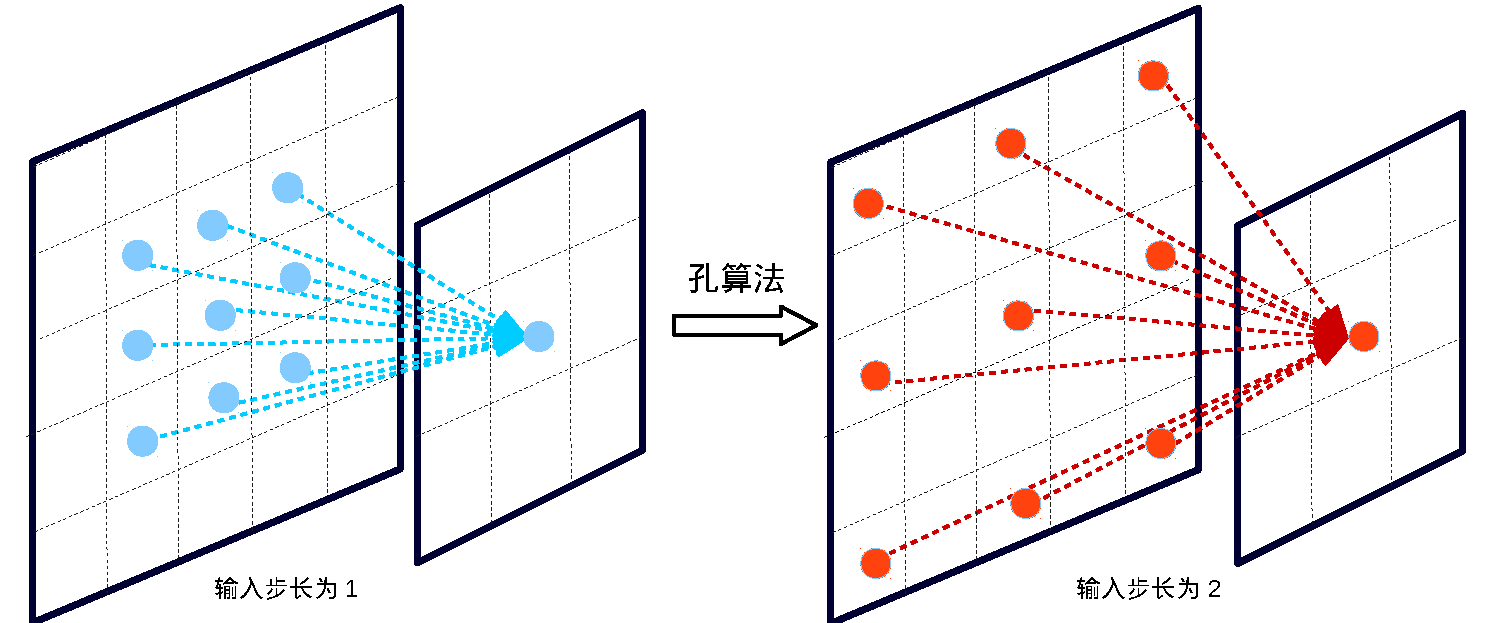
\includegraphics[width=0.7\textwidth]{image/illustration/hole.pdf}
		\caption{"孔算法"示意图}
	\end{figure}
}

\frame{
\frametitle{网格型长短记忆网络部分}
	\vspace{-1em}
    \begin{columns}%[onlytextwidth]
        \begin{column}{0.6\textwidth}
        \vspace{0.2em}
		\begin{figure}
			\centering
			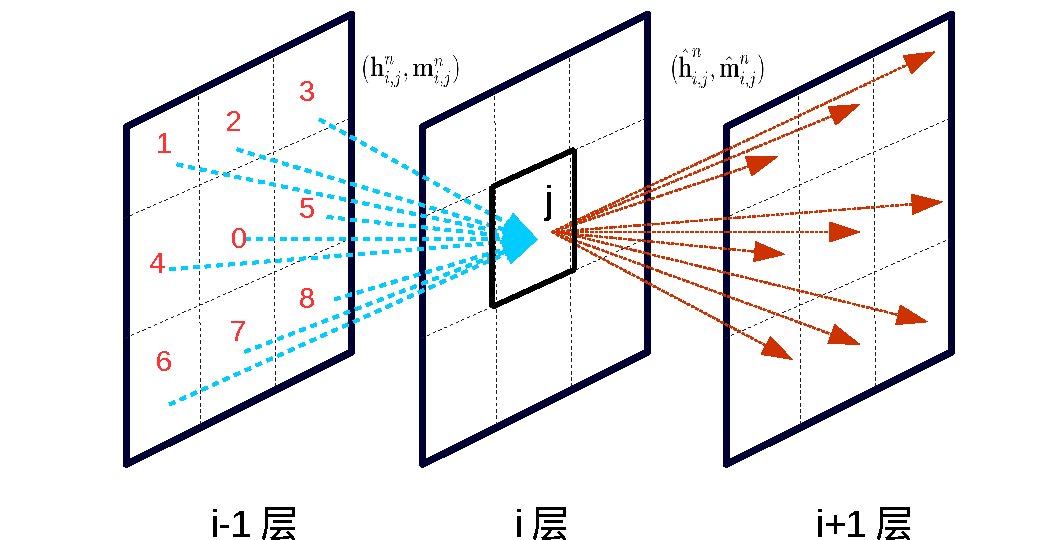
\includegraphics[width=\textwidth]{image/illustration/neighboring.pdf}
			\caption{九维网格型长短记忆网络层之间的通信示意图}
			\label{fig:neighboring}
		\end{figure}
		\end{column} 
		%%%%%%% new column
		\begin{column}{0.5\textwidth}
			\footnotesize
			\vspace{-1.5em}
			\begin{align}
				\begin{split}
				(\hat{\textbf{h}}_{i,j}^0,\hat{\textbf{m}}_{i,j}^0) &= \mbox{LSTM}(\textbf{H}_{i,j},\textbf{m}_{i,j}^0,\textbf{W}_i) \\
				(\hat{\textbf{h}}_{i,j}^1,\hat{\textbf{m}}_{i,j}^1) &= \mbox{LSTM}(\textbf{H}_{i,j},\textbf{m}_{i,j}^1,\textbf{W}_i) \\
				\vdots \\
				(\hat{\textbf{h}}_{i,j}^N,\hat{\textbf{m}}_{i,j}^N) &= \mbox{LSTM}(\textbf{H}_{i,j},\textbf{m}_{i,j}^N,\textbf{W}_i) \\
				\textbf{H}_{i,j} &= [\textbf{h}_{i,j}^0\mbox{ }\textbf{h}_{i,j}^1\mbox{ }...\mbox{ }\textbf{h}_{i,j}^N]^T
				\end{split}
			\end{align}
		\end{column}
    \end{columns}
	\footnotesize
	\vspace{-1em}
	\begin{block}{九维网格型长短记忆网络}
		\vspace{-0.7em}
		\begin{itemize}
			\item 每个位置的预测会受到上一层相邻八邻域特征的影响
			\item 随着层数的堆叠,每一位置将会有更大的感知域。
			\item 网格型长短记忆网络的层数通过实验来确定
		\end{itemize}
	\end{block}
}



\chapter{数据认证方案优化}
本章介绍对第二章提出的多节点联合数据认证机制进行的优化,利用多种方案提升数据认证机制的检测效率,降低节点能量消耗。
4.1节介绍无线传感网节点失效问题,提出了多路径抗节点失效的机制。
4.2节设计动态步长的多节点联合数据认证机制对传感网能量开销进行优化。
\section{多路径抗节点失效机制}
\subsection{数据认证中的节点失效问题}
由于无线传感网部署的环境恶劣,且容易受到攻击,使得节点的稳定性很难保证,整个网络的拓扑结构很容易发生变化。在3.3节中,我们讨论了在拓扑结构变化频率不大的情况下,通过传感器网络自身的维护机制,维护路径节点的上下行相关关系,适应无线传感网拓扑结构的变化。但是在节点失效或者被攻击比较频繁时,无线传感器网络结构变化很快,而原有的维护方案是通过重建路径来完成的,因而通信开销较大,造成大量节点能量损耗。

为了适应节点失效较多,传感网拓扑结构变化较大的情况,我们提出了多路径抗节点失效的方案。通过在初始化阶段预定义若干条不相交路径,对每个节点失效的情况预定义编织路径。但在一个传输阶段,只有一条路径被使用,并进行数据认证。当路径受到攻击,或者节点失效时,使用备用的不相交路径或者编织路径。通过多路径抗节点失效机制,提升了传输路径的稳定性,保证了路径中检测虚假数据报文的性能。

在多路径抗节点失效方案中,我们使用了单向hash链来分配密钥,提升了网络的安全性能,并节省了节点存储密钥的开销。每个节点使用单向hash函数从它的上行相关节点的密钥生成密钥,具体的密钥分配方案将在第五章进行详细描述。
\subsection{多路径抗节点失效机制设计实现}
在多路径抗节点失效机制中,节点上下行相关关系不是研究重点,不再详细介绍,沿用第三章中多跳长路径多节点联合数据认证的方案。我们在多路径抗节点失效机制中,使用了单向hash链来分配密钥,能更好地保证认证机制的安全性,降低节点保存密钥的存储开销。我们的路径抗节点失效机制包括了初始化和密钥分配、数据报文发送、路径中过滤、基站认证、路径选择五个阶段,如图~\ref{fig:MPA}所示:
\begin{figure}[htbp]
  \centering
  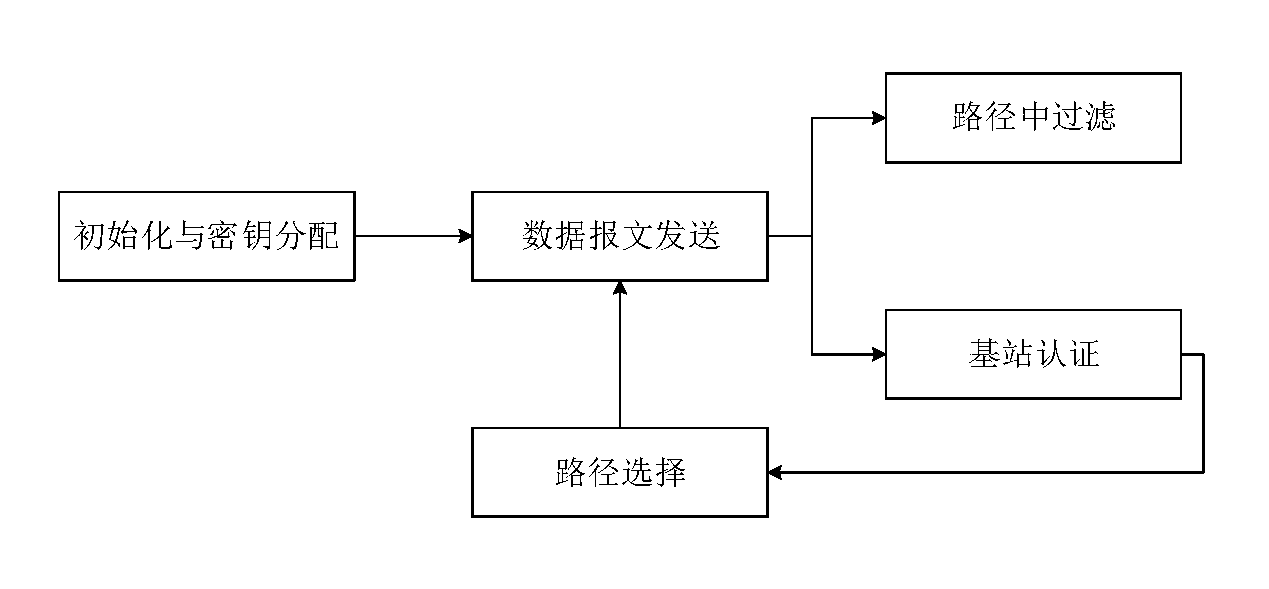
\includegraphics[width=5in]{MPA}
  \caption{多路径抗节点失效机制流程}
  \label{fig:MPA}
\end{figure}
\subsubsection{初始化和密钥分配}
传感器节点被部署到目标监测区域之后,基站会给每个节点生成一个共享密钥,这是每个节点与基站之间的共享密钥$AK_{si}$。然后每个簇通过预定的选举机制选举一个簇头节点,BS通过广播路由请求完成传感器网络的路由发现。

在多节点联合数据认证方案中,我们使用HELLO报文和ACK报文来完成路径发现和上下行相关关系的建立,在簇与BS之间建立一条多跳长路径。在多路径抗节点失效方案中,我们在初始化建立多条不相交长路径以及多条编织路径。虽然有多条路径,在我们的方案中,一次传输过程只会使用一条主路径,其他路径作为网络被攻击时的备选路径。

\begin{figure}[htbp]
  \centering
  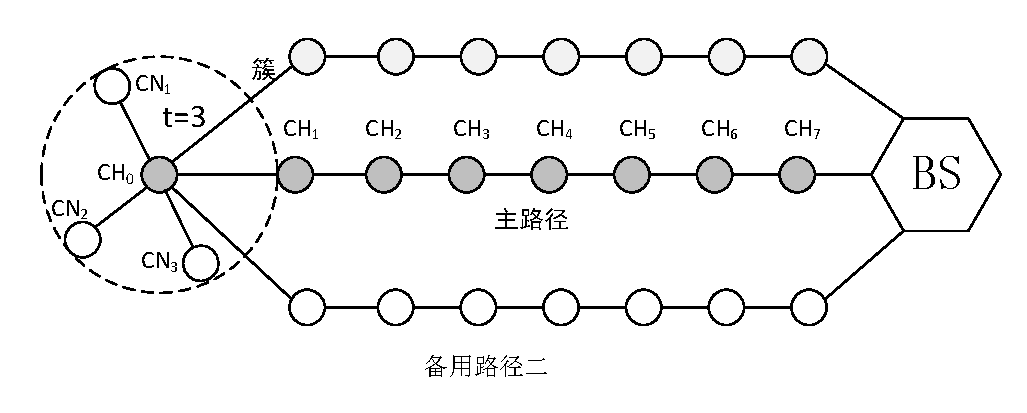
\includegraphics[width=5in]{IHAA1}
  \caption{多路径抗节点失效机制中的不相交路径}
  \label{fig:IHAA1}
\end{figure}
如图~\ref{fig:IHAA1}所示,簇与BS之间建立了3条不相交路径。不相交路径通过以下步骤建立:
\begin{compactitem}
  \item 建立一条簇头与BS之间的主路径。
  \item 建立一条与主路径不相交的,且跳数最短的路径,作为备用路径一。
  \item 建立一条与主路径以及备用路径一不相交的,且跳数最短的路径,作为备用路径二。
\end{compactitem}

\begin{figure}[htbp]
  \centering
  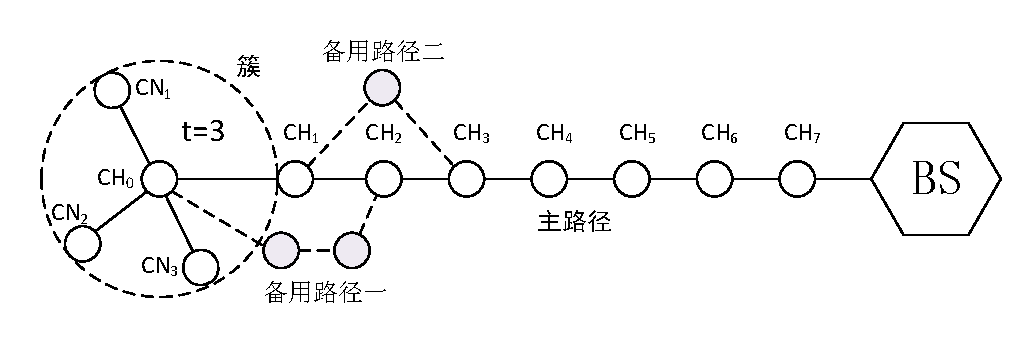
\includegraphics[width=5in]{IHAA2}
  \caption{多路径抗节点失效机制中的编织路径}
  \label{fig:IHAA2}
\end{figure}
如图~\ref{fig:IHAA2}所示,路径上的节点完成备用编织路径的建立。编织路径通过以下步骤建立:
\begin{compactitem}
  \item 建立一条簇头与BS之间的主路径。
  \item 对主路径上的每个节点,寻找不包括该节点的簇与BS之间的最短路径。在图~\ref{fig:IHAA2} 中,第一条编织路径就是不包括节点$CH_1$,从节点$CH_0$到节点$CH_2$之间的编织路径。相似的,第二条编织路径是不包括节点$CH_2$的从节点$CH_1$到节点$CH_3$的编织路径。
\end{compactitem}

\begin{figure}[htbp]
  \centering
  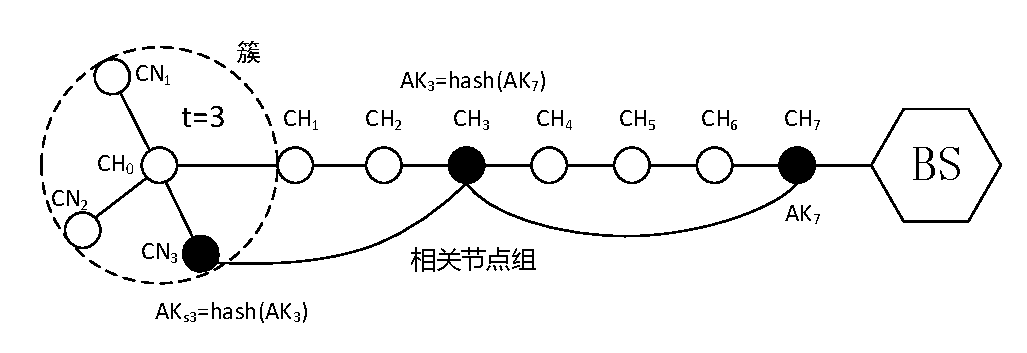
\includegraphics[width=5in]{IHAA3}
  \caption{多路径抗节点失效机制的密钥分配}
  \label{fig:IHAA3}
\end{figure}
在我们的多路径抗节点失效方案中,我们使用了单向hash链来进行密钥分配,如图~\ref{fig:IHAA3}所示。BS给每个上下行相关节点组生成一个$AK$,下行节点使用单向hash函数$H$从上行节点的密钥得到自己的密钥。图~\ref{fig:IHAA3}中所示,节点组\{$CN_3$,$CH_3$,$CH_7$\},距离BS最近的节点$CH_7$从BS获取BS生成的密钥$AK_7$,它的下行节点$CH_3$通过单向hash函数获取密钥$AK_3=H(AK_7)$。类似的,节点$CN_3$获取密钥$AK_{s3}=H(AK_3)$。通过这样的密钥分配,每个节点存储密钥的空间开销变小了,同时节点被攻击时丢失的密钥信息变少了。
\subsubsection{数据报文发送}
同多节点联合数据认证一样,簇节点监测到事件E以后,必须要$t+1$个节点都发出报文才能确认监测到的事件,如果没有至少$t+1$个节点的报文,则认为是无效事件。
簇节点MAC压缩后记作$XMAC(E)$:
\begin{equation}\label{XMAC}
\begin{split}
  XMAC(E)
  &=MAC(AK_{s1},E)\oplus MAC(AK_{s2},E)\oplus MAC(AK_{s3},E)\oplus MAC(AK_{s0},E)
\end{split}
\end{equation}
在多路径抗节点失效方案中,我们使用簇序号$C_i$来标记簇信息,代替原方案中的簇ID集,减小了传输开销。在簇头节点$CH_0$生成的报文R可以记作:
\begin{equation}\label{report1}
\begin{split}
  R=
  & E,C_i,h_0,XMAC(E),\{MAC(AK_{s1},E),\\
  & MAC(AK_{s2},E),MAC(AK_{s3},E),MAC(AK_0,E)\}
\end{split}
\end{equation}
\subsubsection{路径中过滤}
当节点$CH_i$从下行节点收到报文R以后,首先用相邻节点共享密钥对进行认证。然后使用其上下行相关节点的共享密钥对E计算MAC,并更新报文R。对于图~\ref{fig:IHAA3}中的节点$CH_3$,收到来自$CH_2$ 的报文后,首先使用单向hash函数计算得出其下行相关节点的密钥$AK_{s3}=H(AK_3)$。用$AK_{s3}$对事件$E$计算消息认证码$MAC(AK_{s3},E)$,与报文R中的第
$(h_0 - h_i)-((h_0 - h_i)/(t+1))\ast (t+1)=3$ 个相关节点MAC,也就是$MAC(AK_{s3},E)$进行比较,如果不同则丢弃报文R;如果相同则使用密钥$AK_3$ 对事件E计算消息认证码$MAC(AK_3,E)$,并替代原报文R中的$MAC(AK_{s3},E)$,将其转发给下一节点$CH_4$,更新后发送的报文R 为:
\begin{equation}\label{report2}
\begin{split}
  R=
  & E,C_i,h_0,XMAC(E),\{MAC(AK_1,E),\\
  & MAC(AK_2,E),MAC(AK_3,E),MAC(AK_0,E)\}
\end{split}
\end{equation}

\subsubsection{基站认证}
当BS收到报文R后,首先获取报文中的簇序号$C_i$,使用BS与簇$C_i$的节点ID列表中$t+1$个簇节点之间的共享密钥计算MAC,并用XOR 运算计算这$t+1$ 个MAC 的值,与报文R中的XMAC比较,如果不同,则丢弃报文。如果相同,则对事件E作出响应。
\subsubsection{路径选择}
当路径中节点受到攻击时,BS会收集到相应的信息,通过妥协节点检测技术\upcite{c4:mathews2007detecting},BS能确定哪些路径被攻击,妥协节点检测技术不是本文的重点,而是专注于妥协节点检测技术在数据认证中的应用。当BS确定了受攻击的路径以后,切换到未被攻击的备用路径。

同多节点联合数据认证机制中的节点关系维护相比,我们的多路径抗节点失效是通过预先定义备用路径,是一个应对节点攻击的前瞻性安全机制。而多节点联合数据认证机制中的节点维护是一种即时修复的方法,在节点失效或被攻击频率较高时,会造成传感器网络的传输路径不稳定,受攻击的影响更严重,还会造成大量的节点能量消耗。
\subsection{性能分析}
\subsubsection{安全性能分析}
在多跳长路径上多节点联合的数据认证机制中,被捕获节点的限度为$t$,当不少于$t$个节点被捕获,路径中的过滤就有可能无法检测出虚假数据报文。通过建立多跳备用路径和编织路径,多路径抗节点失效机制有更好的安全性能稳定性,在不少于$t$个节点被捕获时,仍能保证数据认证的安全性。

在多路径抗节点失效机制中,使用了基于单向hash链的密钥分配方案,保证了下行节点无法泄露上行节点的密钥。通过降低密钥信息丢失的概率,也提升了数据认证机会的安全性能。
\subsubsection{开销分析}
簇规模为$t+1$时,多路径的建立需要最少$N=(t+1)+d(t+1)$个节点,编织路径的建立需要至少$2(t+1)$个节点。
在提出的多路径抗节点失效机制中,MAC的计算是主要的计算开销,而且多路径抗节点失效机制中,每个节点进行认证前需要使用hash 函数进行密钥计算,使用SHA-1进行2byte的hash函数运算需要$1.52 \mu J$的能量开销。多路径抗节点失效机制需要维护多条备用路径和编织路径,有更高的能量开销,但是在虚假数据报文的比例较高时,因为其稳定的检测率,能明显减小传感网的能量开销。

\section{动态步长多节点联合数据认证}
\subsection{数据认证中的传输开销问题}
在无线传感网的多跳长路径传输中应用我们的多节点联合数据认证机制,能有效保证数据的安全传输,但是数据报文中附带了大量的MAC信息,加重了传感器节点的能量消耗。在规模化无线传感网中,由于传输路径跳数较多,数据传输实时性较高,节点的能量开销较大,因此安全机制的开销优化非常重要。

我们提出了一个动态步长的多节点联合数据认证,在传感器网络节点受攻击影响较小的时候,压缩所传输的报文,降低节点能量消耗,优化无线传感网的开销。
\subsection{动态步长多节点联合数据认证机制设计}
动态步长多节点联合数据认证是在多节点联合数据认证的基础上,对其进行改进,使得通信开销得到优化。
在4.1节中,我们讨论了在传感网拓扑结构变化较大时,使用多路径抗节点失效的机制来保证传感网传输稳定性。对于一条簇到BS之间的传输路径,如果路径比较稳定,则可以通过压缩数据报文的方式来降低传输开销。在我们提出的动态步长多节点联合数据认证机制中,是通过动态调整多节点联合认证中的节点组间隔步长来实现的。

在多节点联合数据认证中,根据步长的动态调整,对数据报文中的相关节点MAC进行相应程度的压缩处理,在路径传输的安全性与路径传输通信开销之间进行平衡,在保证路径安全性的情况下,降低通信开销。如图~\ref{fig:IHAA4}所示,是一个簇节点数为4,步长为3 的多节点联合数据认证。
\begin{figure}[htbp]
  \centering
  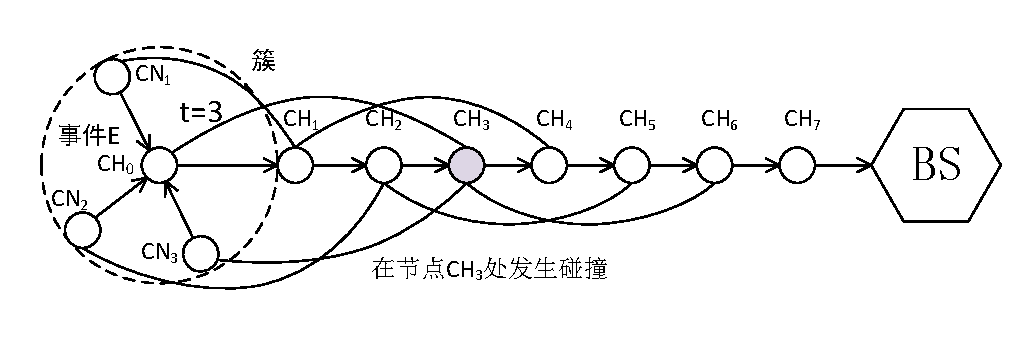
\includegraphics[width=5in]{IHAA4}
  \caption{动态步长多节点联合数据认证}
  \label{fig:IHAA4}
\end{figure}
\subsubsection{面向动态步长多节点联合数据认证的密钥分配}
%密钥分发,节点关系
在动态步长多节点联合数据认证中,我们也使用单向hash链来完成认证密钥的分配。不同于图~\ref{fig:IHAA3}中所示的密钥分配,在步长动态变化时,上下行相关节点组会发生碰撞,也就是不同的簇节点在同一个上下行相关节点组当中。如图~\ref{fig:IHAA4}中,节点$CH_0$和节点$CN_3$在同一个上下行相关节点组中,上行相关节点都是节点$CH_3$。

对于上下行相关节点的碰撞,我们通过对簇内节点添加虚拟的上下行顺序来解决。在如图~\ref{fig:IHAA4}的传输路径上,将4个簇节点的虚拟上下行关系设为$\{CN_3,CN_2,CN_1,CH_0\}$,也即步长为3时,节点$CH_0$是节点$CN_3$的上行相关节点。

\begin{figure}[htbp]
  \centering
  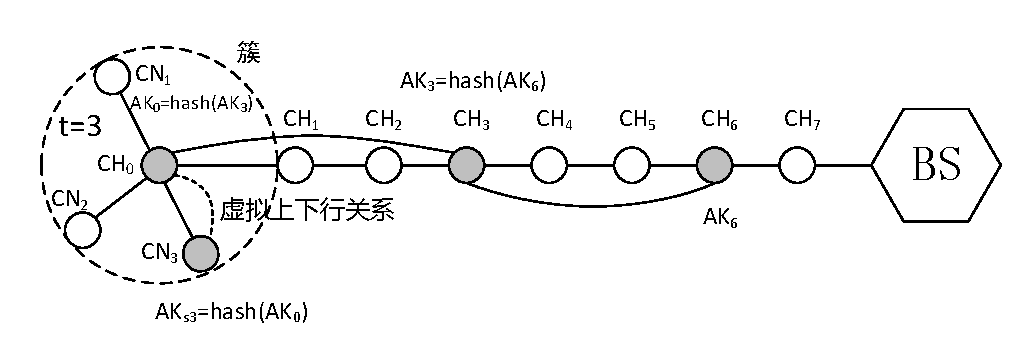
\includegraphics[width=5in]{IHAA5}
  \caption{面向动态步长多节点联合数据认证的密钥分配}
  \label{fig:IHAA5}
\end{figure}

如图~\ref{fig:IHAA5}所示,即为图~\ref{fig:IHAA4}所示的动态步长多节点联合数据认证情景的密钥传输示例。节点$CH_0$和节点$CN_3$都是簇节点,但是在同一个上下行相关节点组内,所以在节点$CH_0$和节点$CN_3$之间虚拟上下行相关关系,节点$CN_3$的密钥从节点$CH_0$的密钥计算而来,$AK_{s3}=H(AK_0)$。
\subsubsection{报文数据压缩传输}
使用单向hash链的密钥分配方案,给虚拟上下行相关节点分配了密钥以后,如图~\ref{fig:IHAA4}的动态步长多节点联合数据认证中,节点$CH_0$ 对簇节点数据进行整合之后的报文R可以表示为:
\begin{equation}\label{report3}
\begin{split}
  R=
  & E,C_i,h_0,XMAC(E),\{MAC(AK_{s1},E),MAC(AK_{s2},E),\\
  & MAC(AK_0,E)\oplus MAC(AK_{s3},E)\}
\end{split}
\end{equation}
其中$MAC(AK_0,E)\oplus MAC(AK_{s3},E)$为节点$CH_0$和节点$CN_3$的簇节点MAC使用XOR运算压缩后的结果。

我们用$p$表示步长,对于$h-h_0\leq p$的节点,在收到报文后,首先计算其下行相关节点的密钥。在图~\ref{fig:IHAA4}的示例中,节点$CH_3$ 收到报文R以后,首先计算下行相关节点的密钥$AK_0=H(AK_3)$。对事件E计算消息认证码$MAC(AK_0,E)$,并与报文R中第
$(h_0 - h_i)-((h_0 - h_i)/p)\ast p=3$个MAC进行比较,如果相同则用$MAC(AK_3,E)$替换之。如果不同则计算间隔一跳的下行相关节点的密钥$AK_{s3}=H(AK_0)$,对事件E计算消息认证码$MAC(AK_{s3},E)$,并与$MAC(AK_0,E)$进行XOR运算,
$MAC(AK_0,E)\oplus MAC(AK_{s3},E)$与报文R中第3个MAC进行比较,如果相同则用$MAC(AK_3,E)$替换之。
如果都不同,则表示是错误数据报文,但是不同于前面提出的方案,我们不将其直接丢弃,而是将$XMAC(E)$置为全0。
对于$h-h_0> p$的节点,同前述方案一样,只进行一次MAC验证。
在经过路径节点的验证后,节点将报文继续转发给上行节点。

\subsubsection{动态步长调整机制}
在BS收到报文以后,会对报文中的$XMAC(E)$进行验证。如果$XMAC(E)$为全0,则说明有错误数据报文在路径中被检测出来,这样说明传输路径的安全水平较低,则BS提高路径的传输步长$p$,这样能提升检测出错误数据报文的概率。如果BS连续收到若干个正常,达到一个阈值以后,我们认为路径是安全的,则BS降低路径的传输步长$p$,减小报文的大小,节约节点的传输能量。
\subsection{性能分析}
动态步长调整机制是建立在基站对路径的安全水平的评价基础上的,当路径的安全水平较高时,调整步长,压缩数据报文大小,降低传输的能量开销;当路径安全水平较低时,维持原有的步长,保证数据认证的安全性能。因此动态步长数据认证机制在安全性能上相比多节点联合数据认证无明显降低。

动态步长数据认证机制有效的在安全性能和能量开销之间进行权衡,在保证基本的安全性能的基础上优化能量开销。
在传感网中的虚假数据较少,也就是路径安全水平较高时,动态步长数据认证机制在能量开销上有明显的优化。

\section{本章小结}
本章针对多节点联合数据认证机制中,节点失效或者受攻击对路径中的节点相关关系的影响,我们提出了多路径抗节点失效的机制,设计实现了相关算法。为了优化多节点联合数据认证的通信开销,我们设计实现了动态步长多节点联合数据认证机制。对两个优化方案,都进行了相关安全性能的分析。




%%
% 结论
% 结论是毕业论文的总结,是整篇论文的归宿,应精炼、准确、完整。结论应着重阐述自己的创造性成果及其在本研究领域中的意义、作用,还可进一步提出需要讨论的问题和建议。
% modifyer: 黄俊杰(huangjj27, 349373001dc@gmail.com)
% update date: 2017-04-13
%%

\chapter{总结与展望}
\section{工作总结}
\section{研究展望}
\section{模板提供的命令}
冒号前面是命令,后面是显示的结果\\

pozhehao(破折号):\pozhehao \sysuspace mybold\{com\}(加粗斜体):\mybold{com} \sysuspace  etoday:\etoday\sysuspace ctoday:\ctoday\sysuspace


用于equation环境的命令

$norm :\norm{t}$

$argmax:\argmax{x}{y}\sysuspace argmin:\argmin{x}{y}$

$varmax:\varmax{x}{y}\sysuspace  varmin:\varmin{x}{y}$

$fncmax:\fncmax{x}{y}\sysuspace  fncmin:\fncmin{x}{y}$

$xxFnorm:\xxFnorm{x}\sysuspace xxFnormSqr:\xxFnormSqr{x}\sysuspace xxFprod:\xxFprod{x}{y}$

$xxOpVec:\xxOpVec{x}\sysuspace xxLprod:\xxLprod{x}{y}\sysuspace xxLprodVec:\xxLprodVec{x}{y}\sysuspace xxTensor:\xxTensor{x}$

$xxBracketY:\xxBracketY{x}\sysuspace xxBracketF:\xxBracketF{x}\sysuspace xxBracketH:\xxBracketH{x}$

\begin{figure}
	\centering
	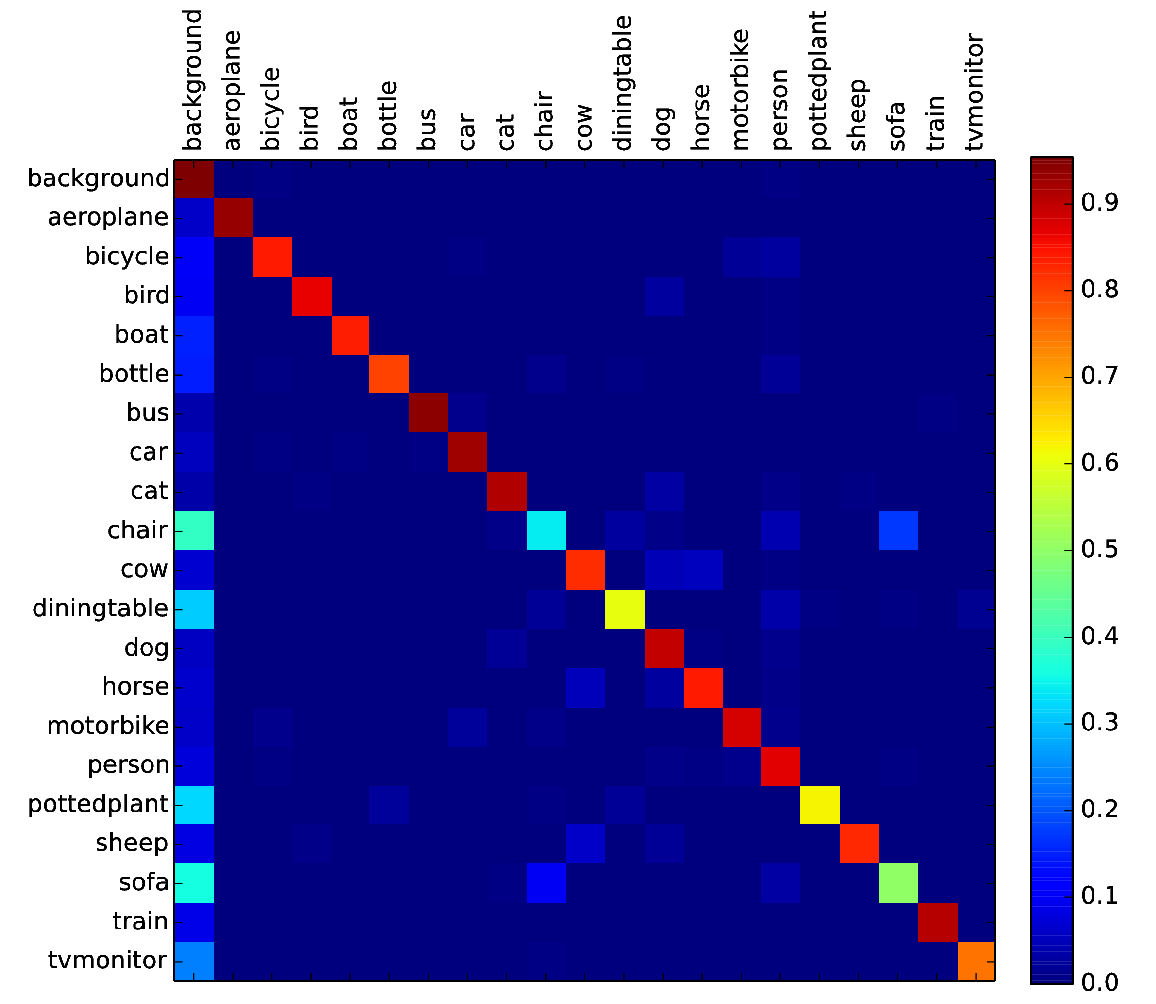
\includegraphics[width=0.5\textwidth]{image/result/confusion.pdf}
	\caption{镶嵌在文中的图像}
	\captionce[图注]{这是测试图注。}{A testing figure legend.}\label{fig:test}
	\label{fig:confusion}
\end{figure}
\section{致谢}
\subsection*{致谢}
\frame{
	\frametitle{致谢}
	\begin{block}{感谢每一个帮助过我的人}
	\begin{itemize}
		\item 首先要感谢的是我的指导老师的悉心指导
		\item 感谢师兄师姐、同学的帮助
		\item 感谢家人的支持
		\item 感谢答辩委员会的聆听和指导
	\end{itemize}
	\end{block}
	\vspace{-1em}
	\note{
		我的展示到此结束,我要感谢我的指导老师,师兄师姐同学,家人还有答辩委员会老师的聆听与指导。谢谢大家
	}
}
\frame{
	\frametitle{Q \& A}
	\begin{block}{Questions?}
	 ~\\ ~\\
	 \center{\Large{Thank you!}}
	 \\ ~\\ ~\\ ~\\ ~\\ 
	\end{block}
	\note{
		现在是问答时间。请问老师们对我的展示有什么疑问?
	}
}


\chapter{总结与展望}
本章对本文完成的研究工作进行总结,针对课题研究中待完善的地方,提出下一步工作的设想。
\section{本文总结}
无线传感网在许多大范围监测领域都有广泛的应用,在环境监测、军事侦察等领域都有规模化的应用。无线传感器节点通常被部署在
环境恶劣的无人值守区域,容易节点受损或者节点受攻击,导致传感网的传输受到严重影响。因此需要对无线传感网中的传输进行认证,保证数据传输的安全性。但是由于无线传感器节点计算能力、存储空间有限,而且节点能量受到限制,因此安全机制的设计必须满足轻量级的要求,以适应传感器节点的限制。我们设计了多跳长路径上多节点联合的数据认证机制,有效利用了数据认证机制保障了传输路径上的安全。

本文主要工作总结如下:
\begin{enumerate}\setlength{\itemsep}{-\itemsep}
  \item 深入研究了无线传感网中数据认证及其密钥分配的理论,分析了它们的发展研究现状,分析了数据认证在无线传感网中的应用,并总结了各种方案的优点和宝贵经验。
  \item 提出了多跳长路径上多节点联合数据认证的模型,设计实现了多跳长路径上多节
        点联合数据认证协议,并设计了路径上节点关系的维护算法,对协议的安全
        性能进行了分析评价。
  \item 针对多跳长路径上多写点联合数据认证协议的不足,对算法进行了优化,提
        出了多路径抗节点失效机制和动态步长多节点联合数据认证机制,并对优化
        方案的安全性能进行了分析评价。
  \item 围绕多跳长路径多节点联合数据认证机制的需求,对密钥分配方案进行了深
        入研究,提出了基于单向 hash 链的密钥分配方案,并对认证中的 MAC 进行
        了研究,提出了适应数据认证机制需求的 MAC 码。
  \item 通过仿真实验验证了本文中提出的方案的安全性能以及优化效果。
\end{enumerate}



\section{未来工作于展望}
本文设计实现的多跳长路径上多节点联合的数据认证机制能够很好地提升了无线传感网数据传输的安全性,取得了一定的成果。但是由于无线传感网本身的复杂性以及部署场景的多样性,我们的机制对不同工作场景下的无线传感网的适应性还需进一步研究,在数据认证的具体算法以及密钥分配等方向还有进一步研究的空间。结合现阶段以及完成的工作,我们未来可做的相关工作有:

\begin{enumerate}\setlength{\itemsep}{-\itemsep}
  \item 本文研究的数据认证机制与无线传感网现有的各层次协议结合还不够,在后续的工作中可以将数据认证机制同其他协议结合起来,例如同网络层的路由协议相结合,将数据认证的相关报文使用路由报文发送。
  \item 针对本文的数据认证机制提出的两个优化方案,虽然在仿真实验环境中已经进行了验证,但在实际的规模化无线传感网中部署比较复杂,可进一步通过搭建真实的传感器节点平台和较大规模无线传感网环境,对相关方案进行针对性的优化。
  \item 密钥分配方案的设计实现还不够完善,需要对相关的算法进行进一步的改进,形成完整的密钥管理机制,并对密钥分配方案的效率和安全性进行分析评价。使用的单向hash函数还有改进的空间,可以进一步压缩其计算开销。
\end{enumerate}






%\chapter{论文正文}
\label{chap:main}
本章将进入论文排版的正文, 按元素分主要包括:
{\kai 字体段落,图片表格,公式定理,参考文献}这几部分。
这个样例文件将包括模板中使用到的所有格式、模板中自定义命令到或者特有的东西,
都将被一一介绍,希望大家在排版自己的学位论文前能细致的看一遍,记住样例的格式和
方法,方便上手。

\section{字体段落}
\label{sec:font}

陈赓(1903年2月27日-1961年3月16日),原名陈庶康,中国湖南湘乡人,军事家。出生将门,其祖父为湘军将领陈翼怀。

Adobe中文字体有四种:

{\kai 楷体\verb|\kai|:陈赓,中国湖南湘乡人,军事家。出生将门,其祖父为湘军将领陈翼怀。%
1952年筹办并任人民解放军军事工程学院第一任院长兼政委,培养国防科技人才。1955年被授予大将军衔。}

{\fs 仿宋\verb|\fs|:陈赓,中国湖南湘乡人,军事家。出生将门,其祖父为湘军将领陈翼怀。%
1952年筹办并任人民解放军军事工程学院第一任院长兼政委,培养国防科技人才。1955年被授予大将军衔。}

{\hei 黑体\verb|\hei|:陈赓,中国湖南湘乡人,军事家。出生将门,其祖父为湘军将领陈翼怀。%
1952年筹办并任人民解放军军事工程学院第一任院长兼政委,培养国防科技人才。1955年被授予大将军衔。}

宋体就是正文字体了。下面测试字体大小,\LaTeX{}默认的列表环境会在
条目之间插入过多的行距,在下面这种情况可能正好,若用户需要
{\kai 正文行距}的列表环境,可以使用compactitem环境,记住这点很重要,不要再
用那种自己修改\verb|itemsep|的傻傻的办法了。
\begin{itemize}
\item[初号] {\song\chuhao 陈赓大将}
\item[小初] {\song\xiaochu 陈赓大将}
\item[一号] {\song\yihao 陈赓大将}
\item[小一] {\song\xiaoyi 陈赓大将}
\item[二号] {\song\erhao 陈赓大将}
\item[小二] {\song\xiaoer 陈赓大将}
\item[三号] {\song\sanhao 陈赓大将}
\item[小三] {\song\xiaosan 陈赓大将}
\item[四号] {\song\sihao 陈赓大将}
\item[小四] {\song\xiaosi 陈赓大将}
\item[五号] {\song\wuhao 陈赓大将}
\item[小五] {\song\xiaowu 陈赓大将}
\end{itemize}

\section{表格明细}
\label{sec:figure}
表格是论文的重要组成部分,我们从简单的表格讲起,到复杂的表格为止。

模板中关于表格的宏包有三个: \textsf{booktabs}、\textsf{array} 和
\textsf{longtabular}。三线表建议使用\textsf{booktabs}中提供的,
包含toprule、midrule 和 bottomrule三条命令,简单干脆!
它们与\textsf{longtable} 能很好的配合使用。下面来看一个表格实例:
\begin{table}[htb]
  \centering
  \begin{minipage}[t]{0.8\linewidth} % 如果想在表格中使用脚注,minipage是个不错的办法
  \caption[模板文件]{模板文件。如果表格的标题很长,那么在表格索引中就会很不美
    观,所以要像 chapter 那样在前面用中括号写一个简短的标题。这个标题会出现在索
    引中。}
  \label{tab:template-files}
    \begin{tabular*}{\linewidth}{lp{10cm}}
      \toprule[1.5pt]
      {\hei 文件名} & {\hei 描述} \\
      \midrule[1pt]
      nudtpaper.ins & \LaTeX{} 安装文件,docstrip\footnote{表格中的脚注} \\
      nudtpaper.dtx & 所有的一切都在这里面\footnote{再来一个}。\\
      nudtpaper.cls & 模板类文件。\\
      nudtpaper.cfg & 模板配置文。cls 和 cfg 由前两个文件生成。\\
      bstutf8.bst   & 参考文献 Bibtex 样式文件。\\
      mynudt.sty    & 常用的包和命令写在这里,减轻主文件的负担。\\
      \bottomrule[1.5pt]
    \end{tabular*}
  \end{minipage}
\end{table}

表 \ref{tab:template-files} 列举了本模板主要文件及其功能,基本上来说论文
中最可能用到的就是这种表格形式了。
请大家注意三线表中各条线对应的命令。这个例子还展示了如何在表格中正确使用脚注。
如果你不需要在表格中插入脚注,可以将minipage环境去掉。
由于\LaTeX{}本身不支持在表格中使用\verb|\footnote|,所以我们不得不将表格放在
小页中,而且最好将表格的宽度设置为小页的宽度,这样脚注看起来才更美观。

另外六院的同学在使用模板时需要使用一种固定宽度(往往是页宽,下面的例子由
rongdonghu提供)的表格,内容需要居中且可以自动调整。
解决办法是自定义了一种\verb|tabularx|中的\textbf{Z}环境,在论文模板中,
该命令已添加到\verb|mynudt.sty|中。下面是这种情况的实例:

\begin{table}[htbp]
\centering
\begin{minipage}[t]{0.9\linewidth}
\caption{Reed Solomon码的典型应用}
\label{tab:RSuse}
\begin{tabularx}{\linewidth}{cZ}
\toprule[1.5pt]
{\hei 应用领域} & {\hei 编码方案}\\
\midrule[1pt]
磁盘驱动器 & RS(32,28,5)码 \footnote{码长为32、维数为28、最小距离为5} \\
CD & 交叉交织RS码(CIRC) \\
DVD & RS(208,192,17)码、RS(182,172,11)码 \\
光纤通信 & RS(255,229,17)码 \\
\bottomrule[1.5pt]
\end{tabularx}
\end{minipage}
\end{table}

我们经常会在表格下方标注数据来源,或者对表格里面的条目进行解释。前面的脚注是一种
不错的方法,如果你不喜欢minipage方法的脚注。
那么完全可以在表格后面自己写注释,比如表~\ref{tab:tabexamp1}。
\begin{table}[htbp]
  \centering
  \caption{复杂表格示例 1}
  \label{tab:tabexamp1}
  \begin{minipage}[t]{0.8\textwidth}
    \begin{tabularx}{\linewidth}{|l|X|X|X|X|}
      \hline
      \multirow{2}*{\backslashbox{x}{y}}  & \multicolumn{2}{c|}{First Half} & \multicolumn{2}{c|}{Second Half}\\
      \cline{2-5}
      & 1st Qtr &2nd Qtr&3rd Qtr&4th Qtr \\
      \hline
      \multirow{2}*{East$^{*}$} &   20.4&   27.4&   90&     20.4 \\
       &   30.6 &   38.6 &   34.6 &  31.6 \\
      West$^{**}$ &   30.6 &   38.6 &   34.6 &  31.6 \\
      \hline
    \end{tabularx}\\[2pt]
    \footnotesize
    *:东部\\
    **:西部
  \end{minipage}
\end{table}

此外,表~\ref{tab:tabexamp1} 同时还演示了另外三个功能:1)通过 \textsf{tabularx} 的
 \texttt{|X|} 扩展实现表格内容自动调整;2)通过命令 \verb|\backslashbox| 在表头部分
插入反斜线(WORD中很简单,但\LaTeX{}做表格需要一定的(极大的)想象力);3)就是
使用\verb|multirow|和\verb|multicolumn|命令。

不可否认 \LaTeX{} 的表格功能没有想象中的那么强大,不过只要你足够认真,足够细致,那么
同样可以排出来非常复杂非常漂亮的表格。可是科技论文中那么复杂表格有什么用呢?
上面那个表格就够用啦。

浮动体的并排放置一般有两种情况:1)二者没有关系,为两个独立的浮动体;2)二者隶属
于同一个浮动体。对表格来说并排表格既可以像表~\ref{tab:parallel1}、表~\ref{tab:parallel2}
使用小页环境,也可以如表~\ref{tab:subtable}使用子表格来做。
图与表同出一源,后面我们将讲解子图(subfloat)的例子。
\begin{table}[htb]
\centering
\noindent\begin{minipage}{0.45\textwidth}
\centering
\caption{第一个并排子表格}
\label{tab:parallel1}
\begin{tabular}{p{2cm}p{2cm}}
\toprule[1.5pt]
111 & 222 \\\midrule[1pt]
222 & 333 \\\bottomrule[1.5pt]
\end{tabular}
\end{minipage}
\begin{minipage}{0.45\textwidth}
\centering
\caption{第二个并排子表格}
\label{tab:parallel2}
\begin{tabular}{p{2cm}p{2cm}}
\toprule[1.5pt]
111 & 222 \\\midrule[1pt]
222 & 333 \\\bottomrule[1.5pt]
\end{tabular}
\end{minipage}
\end{table}
\begin{table}[htbp]
\centering
\caption{并排子表格}
\label{tab:subtable}
\subfloat[第一个子表格]{
\begin{tabular}{p{2cm}p{2cm}}
\toprule[1.5pt]
111 & 222 \\\midrule[1pt]
222 & 333 \\\bottomrule[1.5pt]
\end{tabular}}\hskip2cm
\subfloat[第二个子表格]{
\begin{tabular}{p{2cm}p{2cm}}
\toprule[1.5pt]
111 & 222 \\\midrule[1pt]
222 & 333 \\\bottomrule[1.5pt]
\end{tabular}}
\end{table}

如果您要排版的表格长度超过一页,那么推荐使用\textsf{longtable}命令。
这里随便敲入一些无关的文字,使得正文看上去不是那么的少。
表~\ref{tab:performance} 就是 \textsf{longtable} 的简单示例。
\begin{longtable}[c]{c*{6}{r}}
\caption{实验数据}\label{tab:performance}\\
\toprule[1.5pt]
 测试程序 & \multicolumn{1}{c}{正常运行} & \multicolumn{1}{c}{同步}
& \multicolumn{1}{c}{检查点}   & \multicolumn{1}{c}{卷回恢复}
& \multicolumn{1}{c}{进程迁移} & \multicolumn{1}{c}{检查点} 	\\
& \multicolumn{1}{c}{时间 (s)} & \multicolumn{1}{c}{时间 (s)}
& \multicolumn{1}{c}{时间 (s)} & \multicolumn{1}{c}{时间 (s)}
& \multicolumn{1}{c}{时间 (s)} &  文件(KB)			\\
\midrule[1pt]%
\endfirsthead%

\multicolumn{7}{c}{续表~\thetable\hskip1em 实验数据}\\

\toprule[1.5pt]
 测试程序 & \multicolumn{1}{c}{正常运行} & \multicolumn{1}{c}{同步}
& \multicolumn{1}{c}{检查点}   & \multicolumn{1}{c}{卷回恢复}
& \multicolumn{1}{c}{进程迁移} & \multicolumn{1}{c}{检查点} 	\\
& \multicolumn{1}{c}{时间 (s)} & \multicolumn{1}{c}{时间 (s)}
& \multicolumn{1}{c}{时间 (s)} & \multicolumn{1}{c}{时间 (s)}
& \multicolumn{1}{c}{时间 (s)} &  文件(KB)			\\
\midrule[1pt]%
\endhead%
\hline%

\multicolumn{7}{r}{续下页}%

\endfoot%
\endlastfoot%
CG.A.2 & 23.05   & 0.002 & 0.116 & 0.035 & 0.589 & 32491  \\
CG.A.4 & 15.06   & 0.003 & 0.067 & 0.021 & 0.351 & 18211  \\
CG.A.8 & 13.38   & 0.004 & 0.072 & 0.023 & 0.210 & 9890   \\
CG.B.2 & 867.45  & 0.002 & 0.864 & 0.232 & 3.256 & 228562 \\
CG.B.4 & 501.61  & 0.003 & 0.438 & 0.136 & 2.075 & 123862 \\
CG.B.8 & 384.65  & 0.004 & 0.457 & 0.108 & 1.235 & 63777  \\
MG.A.2 & 112.27  & 0.002 & 0.846 & 0.237 & 3.930 & 236473 \\
MG.A.4 & 59.84   & 0.003 & 0.442 & 0.128 & 2.070 & 123875 \\
MG.A.8 & 31.38   & 0.003 & 0.476 & 0.114 & 1.041 & 60627  \\
MG.B.2 & 526.28  & 0.002 & 0.821 & 0.238 & 4.176 & 236635 \\
MG.B.4 & 280.11  & 0.003 & 0.432 & 0.130 & 1.706 & 123793 \\
MG.B.8 & 148.29  & 0.003 & 0.442 & 0.116 & 0.893 & 60600  \\
LU.A.2 & 2116.54 & 0.002 & 0.110 & 0.030 & 0.532 & 28754  \\
LU.A.4 & 1102.50 & 0.002 & 0.069 & 0.017 & 0.255 & 14915  \\
LU.A.8 & 574.47  & 0.003 & 0.067 & 0.016 & 0.192 & 8655   \\
LU.B.2 & 9712.87 & 0.002 & 0.357 & 0.104 & 1.734 & 101975 \\
LU.B.4 & 4757.80 & 0.003 & 0.190 & 0.056 & 0.808 & 53522  \\
LU.B.8 & 2444.05 & 0.004 & 0.222 & 0.057 & 0.548 & 30134  \\
EP.A.2 & 123.81  & 0.002 & 0.010 & 0.003 & 0.074 & 1834   \\
EP.A.4 & 61.92   & 0.003 & 0.011 & 0.004 & 0.073 & 1743   \\
EP.A.8 & 31.06   & 0.004 & 0.017 & 0.005 & 0.073 & 1661   \\
EP.B.2 & 495.49  & 0.001 & 0.009 & 0.003 & 0.196 & 2011   \\
EP.B.4 & 247.69  & 0.002 & 0.012 & 0.004 & 0.122 & 1663   \\
EP.B.8 & 126.74  & 0.003 & 0.017 & 0.005 & 0.083 & 1656   \\
\bottomrule[1.5pt]
\end{longtable}

另外,有的同学不想让某个表格或者图片出现在索引里面,那么请使用命令 \verb|\caption*{}|,
这个命令不会给表格编号,也就是出来的只有标题文字而没有“表~XX”,“图~XX”,否则
索引里面序号{\kai 不连续}就显得不伦不类,这也是 \LaTeX{} 里星号命令默认的规则。

%\section{绘图插图}
%
%本模板不再预先装载任何绘图包(如 \textsf{pstricks,pgf} 等),完全由你自己来决定。
%个人觉得 \textsf{pgf} 不错,不依赖于 Postscript。此外还有很多针对 \LaTeX{} 的
% GUI 作图工具,如 XFig(jFig), WinFig, Tpx, Ipe, Dia, Inkscape, LaTeXPiX,
%jPicEdt 等等。本人强烈推荐\textsf{Ipe}。
%
%一般图形都是处在浮动环境中。之所以称为浮动是指最终排版效果图形的位置不一定与源文
%件中的位置对应,这也是刚使用 \LaTeX{} 同学可能遇到的问题。
%如果要强制固定浮动图形的位置,请使用 \textsf{float} 宏包,
%它提供了 \texttt{[H]}(意思是图片就给我放在这里\textcolor{red}{H}ere)参数,
%但是除非特别需要,不建议使用\texttt{[H]},而是推荐使用\texttt{[htbp]},
%给\LaTeX{}更多选择。比如图~\ref{fig:ipe}。
%\begin{figure}[htbp] % use float package if you want it here
%  \centering
%  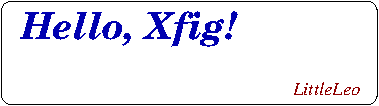
\includegraphics[width=3in]{hello}
%  \caption{利用IPE制图}
%  \label{fig:ipe}
%\end{figure}
%
%若子图共用一个计数器,
%那么请看图~\ref{fig:big1},它包含两个小图,分别是图~\ref{fig:subfig1}
%和图~\ref{fig:subfig2}。这里推荐使用\verb|\subfloat|,{\bf 不要再用}
%\verb|\subfigure|和\verb|\subtable|。
%\begin{figure}[htb]
%  \centering%
%  \subfloat[第一个小图形]{%
%    \label{fig:subfig1}
%    \includegraphics[height=2cm]{xh}}\hspace{4em}%
%  \subfloat[第二个小图形。如果标题很长的话,它会自动换行,这个 caption 就是这样的例子]{%
%    \label{fig:subfig2}
%    \includegraphics[height=2cm]{xhh}}
%  \caption{包含子图形的大图形}
%  \label{fig:big1}
%\end{figure}
%
%而下面这个例子显示并排$3\times2$的图片,见图\ref{fig:subfig:3x2}:
%\begin{figure}[htb]
%\centering
%\subfloat[]{\includegraphics[width=.27\textwidth]{typography}} \qquad
%\subfloat[]{\includegraphics[width=.27\textwidth]{typography}} \qquad
%\subfloat[]{\includegraphics[width=.27\textwidth]{typography}} \qquad
%\subfloat[]{\includegraphics[width=.27\textwidth]{typography}} \qquad
%\subfloat[]{\includegraphics[width=.27\textwidth]{typography}} \qquad
%\subfloat[]{\includegraphics[width=.27\textwidth]{typography}}
%\caption{并排图片}
%\label{fig:subfig:3x2}
%\end{figure}
%
%要注意,图\ref{fig:subfig:3x2}例中
%\texttt{qquad}相当于\verb|\hspace{2em}|,也就是2个字符的宽度,约0.08倍页宽,
%图片宽度设定为0.27倍页宽是合适的;在该环境中,尽量不要手动换行,所以,不妨自己计算一下!
%
%如果要把编号的两个图形并排,那么小页(minipage)就非常有用了,可以分别参考
%图\ref{fig:parallel1}和图\ref{fig:parallel2}。其实这个例子和表格一节中并排
%放置的表格一摸一样。
%\begin{figure}[htb]
%\begin{minipage}{0.48\textwidth}
%  \centering
%  \includegraphics[height=1.2cm]{xhh}
%  \caption{并排第一个图}
%  \label{fig:parallel1}
%\end{minipage}\hfill
%\begin{minipage}{0.48\textwidth}
%  \centering
%  \includegraphics[height=1.2cm]{xhh}
%  \caption{并排第二个图}
%  \label{fig:parallel2}
%\end{minipage}
%\end{figure}
%
%图形就说这么多,因为大家在写论文是遇到的最大问题不是怎么把图插进去,
%而是怎样做出专业的、诡异的、震撼的图片来,记得在这时参考前面推荐的那
%些工具吧,当然必不可少的是Matlab了,至于如何加入中文标注、支持中文等等
%可以上网去查,但这里{\kai 推荐一点},用好export命令,使得插入图片时尽可能的不要
%缩放,保证图文的一致性。

\section{公式定理}
\label{sec:equation}
贝叶斯公式如式~(\ref{equ:chap1:bayes}),其中$p(y|\mathbf{x})$为后验;
$p(\mathbf{x})$为先验;分母$p(\mathbf{x})$ 为归一化因子,这是
实际应用中十分恐怖的一个积分式。
\begin{equation}
\label{equ:chap1:bayes}
p(y|\mathbf{x}) = \frac{p(\mathbf{x},y)}{p(\mathbf{x})}=
\frac{p(\mathbf{x}|y)p(y)}{p(\mathbf{x})}
\end{equation}

论文里面公式越多,\TeX{} 就越 happy。再看一个 \textsf{amsmath} 的例子:
\newcommand{\envert}[1]{\left\lvert#1\right\rvert}
\begin{equation}\label{detK2}
\det\mathbf{K}(t=1,t_1,\dots,t_n)=\sum_{I\in\mathbf{n}}(-1)^{\envert{I}}
\prod_{i\in I}t_i\prod_{j\in I}(D_j+\lambda_jt_j)\det\mathbf{A}
^{(\lambda)}(\overline{I}|\overline{I})=0.
\end{equation}

大家在写公式的时候一定要好好看\textsf{amsmath}的文档,并参考模板中的用法:
\begin{multline*}%\tag{[b]} % 这个出现在索引中的
\int_a^b\biggl\{\int_a^b[f(x)^2g(y)^2+f(y)^2g(x)^2]
 -2f(x)g(x)f(y)g(y)\,dx\biggr\}\,dy \\
 =\int_a^b\biggl\{g(y)^2\int_a^bf^2+f(y)^2
  \int_a^b g^2-2f(y)g(y)\int_a^b fg\biggr\}\,dy
\end{multline*}

再看\ref{equ:split}:
\begin{equation}\label{equ:split}
\begin{split}
C(z) &= [z^n] \biggl[\frac{e^{3/4}}{\sqrt{1-z}} +
e^{-3/4}(1-z)^{1/2} + \frac{e^{-3/4}}{4}(1-z)^{3/2}
+ O\Bigl( (1-z)^{5/2}\Bigr)\biggr] \\
&= \frac{e^{-3/4}}{\sqrt{\pi n}} - \frac{5e^{-3/4}}{8\sqrt{\pi
n^3}} + \frac{e^{-3/4}}{128 \sqrt{\pi n^5}} +
O\biggl(\frac{1}{\sqrt{\pi
n^7}}\biggr)
\end{split}
\end{equation}

当然了,数学中必不可少的是定理和证明:
\begin{theorem}
  \label{chapTSthm:rayleigh solution}
  假定 $X$ 的二阶矩存在:
  \begin{equation}
         O_R(\mathbf{x},F)=\sqrt{\frac{\mathbf{u}_1^T\mathbf{A}\mathbf{u}_1} {\mathbf{u}_1^T\mathbf{B}\mathbf{u}_1}}=\sqrt{\lambda_1},
  \end{equation}
  其中 $\mathbf{A}$ 等于 $(\mathbf{x}-EX)(\mathbf{x}-EX)^T$,$\mathbf{B}$ 表示协方差阵 $E(X-EX)(X-EX)^T$,$\lambda_1$
$\mathbf{u}_1$是$\lambda_1$对应的特征向量,
\end{theorem}

对于希腊符号使用\verb|mathbf|命令可能有些问题,所以建议对符号
用\verb|bm|加粗,记得用\verb|\up<greek>|切换正体符号,下面看几个例子:
\verb|\gamma|斜体代表变量$\gamma$,\verb|\bm{\upgamma}|正体代表向量$\bm{\upgamma}$,
。\verb|\Gamma|正体代表操作符号$\Gamma$,
\verb|\bm{\Gamma}|正体粗体代表矩阵形式$\bm{\Gamma}$,
\verb|\varGamma|斜体代表变量$\varGamma$。另外对于大小写斜体的加粗可以见$\bm{\gamma}$和$\bm{\varGamma}$,
但是这两种科技论文中很少出现,这里只做测试。
非符号普通向量就用\verb|\mathbf|吧:$\mathbf{x}_k,\mathbf{X}_k$。
完整测试如下$\omega,\bm{\omega},\upomega,\bm{\upomega},\Omega,\bm{\Omega},\varOmega,\bm{\varOmega}$。

\begin{proof}
上述优化问题显然是一个Rayleigh商问题。我们有
  \begin{align}
     O_R(\mathbf{x},F)=\sqrt{\frac{\mathbf{u}_1^T\mathbf{A}\mathbf{u}_1} {\mathbf{u}_1^T\mathbf{B}\mathbf{u}_1}}=\sqrt{\lambda_1},
 \end{align}
 其中 $\lambda_1$ 下列广义特征值问题的最大特征值:
$$
\mathbf{A}\mathbf{z}=\lambda\mathbf{B}\mathbf{z}, \mathbf{z}\neq 0.
$$
 $\mathbf{u}_1$ 是 $\lambda_1$对应的特征向量。结论成立。
\end{proof}

下面来看看算法环境的定义和使用。
我们知道,故障诊断的最终目的,是将故障定位到部件,而由于信号--部件依赖矩阵的存在,因此,实质性的工作是找出由故障部件发出异常信号,
不妨称为源异常信号,而如前所述,源异常信号与异常信号依赖矩阵$\mathbf{S_a}$的全零列是存在一一对应的关系的。因此,我们只要获得了$\mathbf{S_a}$的全零列的相关信息,
也就获得了源异常信号的信息,从而能进一步找到故障源。
通过以上分析,我们构造算法\ref{alg53},用于实现非回路故障诊断。
\begin{algorithm}[htbp]
  \caption{非回路故障诊断算法}
  \label{alg53}
  \begin{algorithmic}[1]
    \REQUIRE 信号--部件依赖矩阵$\mathbf{A}$,信号依赖矩阵$\mathbf{S}$,信号状态向量$\alpha$
    \ENSURE 部件状态向量$\gamma$
    \STATE $\mathbf{P}\leftarrow\left(<\alpha>\right)$
    \STATE $\mathbf{S_{a}}\leftarrow\mathbf{P^T}\mathbf{S}\mathbf{P}$
    \FOR{$i=1$ to $S_a$的阶数$m$}
    \STATE $s_i\leftarrow s_i$的第$i$个行向量
    \ENDFOR
    \STATE $\beta_a\leftarrow\lnot \left(s_1\lor s_2\lor \cdots\lor s_m\right)^T$
    \STATE $\beta\leftarrow\mathbf{P}\beta_a$
    \STATE $\gamma\leftarrow\mathbf{A}\beta$
  \end{algorithmic}
\end{algorithm}

第一类故障回路推理与非回路故障推理是算法基本相同,稍微不同的是$\beta_a$的计算。因为第一类故障回路中的信号全部可能是源异常信号,因此我们不必计算
$\beta_a=\lnot \left(\left[s_1\lor s_2\lor \cdots\lor s_m\right]^T\right)$,而直接取$\beta_a=\underbrace{\left[\begin{array}{cccc}1&1&\cdots&1\end{array}\right]^T}_m$,将$\beta_a$代入
算法\ref{alg53},有
\[\beta=\mathbf{P}\beta_a=\mathbf{P}\underbrace{\left[\begin{array}{cccc}1&1&\cdots&1\end{array}\right]^T}_m=\alpha\]
因此一类故障回路的推理算法变得相当简单,例如算法\ref{alg54}
\begin{algorithm}[htbp]
  \caption{第一类故障回路诊断算法}
  \label{alg54}
  \begin{algorithmic}[1]
    \REQUIRE 信号--部件依赖矩阵$\mathbf{A}$,信号状态向量$\alpha$
    \ENSURE 部件状态向量$\gamma$
    \STATE $\gamma\leftarrow\mathbf{A}\alpha$
  \end{algorithmic}
\end{algorithm}

\section{参考文献}
\label{sec:bib}
当然参考文献可以直接写 bibitem,虽然费点功夫,但是好控制,各种格式可以自己随意改
写,在nudtpaper里面,建议使用JabRef编辑和管理文献,再结合\verb|bstutf8.bst|,
对中文的支持非常不错,格式也很规范。

\section{代码高亮}
有些时候我们需要在论文中引入一段代码,用来衬托正文的内容,或者体现关键思路的实现。
在模板中,统一使用\texttt{listings}宏包,并且设置了基本的内容格式,并建议用户只
使用三个接口,分别控制:编程语言,行号以及边框。简洁达意即可,下面分别举例说明。

首先是设定语言,来一个C的,使用的是默认设置:
\begin{lstlisting}[language=C]
void sort(int arr[], int beg, int end)
{
  if (end > beg + 1)
  {
    int piv = arr[beg], l = beg + 1, r = end;
    while (l < r)
    {
      if (arr[l] <= piv)
        l++;
      else
        swap(&arr[l], &arr[--r]);
    }
    swap(&arr[--l], &arr[beg]);
    sort(arr, beg, l);
    sort(arr, r, end);
  }
}
\end{lstlisting}

当我们需要高亮Java代码,不需要行号,不需要边框时,可以:
\begin{lstlisting}[language=Java,numbers=none,frame=none]
// A program to display the message
// "Hello World!" on standard output

public class HelloWorld {

   public static void main(String[] args) {
      System.out.println("Hello World!");
   }

}   // end of class HelloWorld
\end{lstlisting}

细心的用户可能发现,行号被放在了正文框之外,事实上这样是比较美观的,
如果有些用户希望在正文框架之内布置所有内容,可以:
\begin{lstlisting}[language=perl,xleftmargin=2em,framexleftmargin=1.5em]
#!/usr/bin/perl
print "Hello, world!\n";
\end{lstlisting}

好了,就这么多,\texttt{listings}宏包的功能很强大也很复杂,如果需要自己定制,
可以查看其手册,耐心阅读总会找到答案。
\textbf{注意:} 当前代码环境中文注释的处理还不是很完善,对于注释请妥善处理。
在本模板中,推荐算法环境或者去掉中文的listings代码环境。
如果需要包含中文注释,不要求代码高亮,
就用\texttt{code}环境,这个环境是Verbatim的定制版,简单有效,
调用的是fancyvbr宏包,用户可在mynudt.sty中修改它的外观等等。
这里我们还可以给代码加上标签。
\begin{code}[label=hello.c]
public class HelloWorld {
   public static void main(String[] args) {
      System.out.println("Hello World!");
   }
}   // 世界,你好!
\end{code}

\section{符号列表}

{\hei 前面的话:}{\kai\color{blue}
2.2版本后默认使用nomencl环境,如果你还是希望使用传统的\verb|definition.tex|,那么只需注释掉
顶层文件中的nomenclature即可。}

符号列表使用的是\verb|nomencl|包,自己简单定制了下,使用方法分为四步:
\begin{compactenum}
\item 将\verb|\makenomenclature|语句放在正文前,即\verb|\begin{document}|前面;
\item 将\verb|\printnomenclature|放在论文中,我在例子中将符号列表放在了英文摘要的
后面,正文第一章的前面,当然,你可以根据自己的需要或者教研室的规范放置在合理的位置上,
为了页面引用的正确,在这句话前面放上\verb|\cleardoublepage|;
\item 使用\verb|\nomenclature|命令在论文的各个位置上添加符号定义,语法后面会讲到;
\item 编译。编译需要首先运行一遍xelatex,之后运行
\begin{code}
makeindex -s nomencl.ist -o thesis.nls thesis.nlo
\end{code}
\end{compactenum}

你可以把这句编译命令放在\verb|makepdf.bat|中第一个\verb|xelatex thesis|下面。然后
双击\verb|makepdf.bat|就可以了,论文模板中已经为你添加上了,如果你强烈不想使用
nomencl环境,只要把它注释掉(前面加\verb|rem|)就可以。
另外,由于我使用的是VIM来编辑\TeX{}代码,具体到每个编辑器(诸如WinEDT,TeXWorks等)
如何设定该命令的快捷按钮,诸位可以搜索网上的教程。

下面简单说明下\verb|\nomenclature|命令,语法为。这里插入一些随机的文字,希望
对你在阅读帮助中的思维没有什么不良的影响。
\begin{code}
\nomenclature[<prefix>]{<symbol>}{<desc>}{<null>}
\end{code}
\verb|nomencl|模板的默认排序方法可能(大多都)不满足要求,
论文模板里,我们通过设定\verb|<prefix>|来实现符号列表的排序。
它分为两部分,比如如\verb|[Aa]|,第一个字母的含义是:
\begin{compactitem}
\item[`A'] 符号归为拉丁字母
\item[`G'] 希腊字母
\item[`X'] 上标
\item[`Z'] 下标
\end{compactitem}
每个标识后边的字幕\verb|a-z|作为当前符号组内的排列顺序,比如$\beta$就可以写成
\verb|[Gb]|,诸如此类。当然你一定注意到了,这个排序分组的设定只是为了记忆
方便,并不是强制的,因此你可以有自己的方案,比如Z是Greek,
R是Roman什么的,只要统一就好,只需记住,组间排列是按字母顺序排的。

注意符号表分四列,前三列的含义与命令中相同,
最后一列是符号定义时所在的页码。效果看例子,对于下式:
\begin{equation}\label{eq:heatflux}
   \dot{Q} = k \cdot A \cdot \Delta T
\end{equation}%
\nomenclature[Aq]{$\dot{Q}$}{heat flux}{}%
\nomenclature[Ak]{$k$}{overall heat transfer coefficient,式\eqref{eq:ohtc}}{}%
\nomenclature[Aa]{$A$}{area}{}%
\nomenclature[Al]{$L$}{length}{}%
\nomenclature[At]{$T$}{temperature}{}%
\nomenclature[At]{$\Delta T$}{temperature difference}{}%
\nomenclature[Gr]{$\gamma$}{中文测试, 以及一句很长的物理意义,很有可能超过当前栏的宽度,主要目的是看一看会不会出现某些异常情况。}{}%

或者:
\begin{equation}\label{eq:ohtc}
    \frac{1}{k} = \left[\frac{1}{\alpha _{\mathrm{i}}\,r_{\mathrm{i}}} +
    \sum^n_{j=1}\frac{1}{\lambda _j}\,
    \ln \frac{r_{\mathrm{a},j}}{r_{\mathrm{i},j}} +
    \frac{1}{\alpha _{\mathrm{a}}\,
    r_{\mathrm{a}}}\right] \cdot r_{\mathrm{reference}}
\end{equation}%
\nomenclature[Ga]{$\alpha$}{convection heat transfer coefficient}{}%
\nomenclature[Zi]{i}{in}{}%
\nomenclature[Gl]{$\lambda$}{thermal conductivity}{}%
\nomenclature[Za]{a}{out}{}%
\nomenclature[Zn]{$n$}{number of walls}{}%
\nomenclature[Zj]{$j$}{running parameter}{}%

{\hei 注意事项:}{\kai 模板中定制的nomencl格式在mynudt.sty中,默认是三栏的,分别是:
``符号'',``定义'',``首次出现页码'',
注意这里的符号列表都没有单位,如果你需要额外的栏输入单位(呵呵,聪明的读者可能看出来
了,\verb|nomenclature|命令最后一个是空的,就是用来让你赋予她各种意义的)。
此时就需要你有一点点动手能力了(其实只要会修改表格就行),
方法很简单,比如需要添加``国际单位制''这一栏,则
\begin{compactenum}
\item 论文中\verb|\nomenclature|命令的第三个参数就让他代表单位,也可留空;
\item 将\verb|mynudt.sty|中longtable的表头添加``国际单位制''几个字,
你也可以取其他的名字,放在那个{\kai 应该出现的}位置上;
\item 由于增加了5个字,就把前面栏的宽度数字减5,同时设定第三栏宽度为5,
注意这一步需要你自己调整,记得不要让表格超出边界就行。
\end{compactenum}
}

\section{中文习惯}
\label{sec:chinese}

对于itermize过大的行间距,用户可以使用compactitem环境来替代,但是模板中不进行默认替代,
因为只有用户真正发现列表不好看才会找到这里,而且在示例文件中,
陈赓大将那个列表环境如果压缩了行距会很不好看。谢谢ZhangLei的建议!

{\hei 一个重要的提示:}
作者自己的定义命令、包等,不要放在模板里面,请放到\verb|mynudt.sty|
中,这样模板时,只要覆盖\verb|nudtpaper.cls|即可。

中文破折号为一个两个字宽垂直居中的直线,输入法直接得到的破折号是两个断开的小短线
(——),这看起来不舒服。所以模板中定义了一个破折号的命令 \verb|\pozhehao|,请看:

厚德博学,强军兴国\hfill \pozhehao{}国防科大校训



%%% Local Variables:
%%% mode: latex
%%% TeX-master: "../main"
%%% End:

\begin{ack}
  衷心感谢导师 xxx 教授和物理系 xxx 副教授对本人的精心指导。他们的言传身教将使
  我终生受益。

  在美国麻省理工学院化学系进行九个月的合作研究期间,承蒙 xxx 教授热心指导与帮助,不
  胜感激。感谢 xx 实验室主任 xx 教授,以及实验室全体老师和同学们的热情帮助和支
  持!本课题承蒙国家自然科学基金资助,特此致谢。

  感谢 \ucasthesis,它的存在让我的论文写作轻松自在了许多,让我的论文格式规整漂亮了
  许多。
\end{ack}


\cleardoublepage
\phantomsection
\addcontentsline{toc}{chapter}{参考文献}
\bibliographystyle{bstutf8}
\bibliography{ref/refs}

\resumeitem{个人简历:}
\noindent xxxx 年 xx 月 xx 日出生于 xx 省 xx 县。\\
\noindent xxxx 年 9 月考入 xx 大学 xx 系 xx 专业,xxxx 年 7 月本科毕业并获得 xx 学士学位。\\
\noindent xxxx 年 9 月免试进入 xx 大学 xx 系攻读 xx 学位至今。

\resumeitem{发表论文:} % 发表的和录用的合在一起
\begin{enumerate}[{[}1{]}]
\item Yang Y, Ren T L, Zhang L T, et al. Miniature microphone with silicon-
  based ferroelectric thin films. Integrated Ferroelectrics, 2003,
  52:229-235. (SCI 收录, 检索号:758FZ.)
\item 杨轶, 张宁欣, 任天令, 等. 硅基铁电微声学器件中薄膜残余应力的研究. 中国机
  械工程, 2005, 16(14):1289-1291. (EI 收录, 检索号:0534931 2907.)
\item 杨轶, 张宁欣, 任天令, 等. 集成铁电器件中的关键工艺研究. 仪器仪表学报,
  2003, 24(S4):192-193. (EI 源刊.)
\item Yang Y, Ren T L, Zhu Y P, et al. PMUTs for handwriting recognition. In
  press. (已被 Integrated Ferroelectrics 录用. SCI 源刊.)
\item Wu X M, Yang Y, Cai J, et al. Measurements of ferroelectric MEMS
  microphones. Integrated Ferroelectrics, 2005, 69:417-429. (SCI 收录, 检索号
  :896KM.)
\item 贾泽, 杨轶, 陈兢, 等. 用于压电和电容微麦克风的体硅腐蚀相关研究. 压电与声
  光, 2006, 28(1):117-119. (EI 收录, 检索号:06129773469.)
\item 伍晓明, 杨轶, 张宁欣, 等. 基于MEMS技术的集成铁电硅微麦克风. 中国集成电路, 
  2003, 53:59-61.
\end{enumerate}

\resumeitem{研究成果:} % 有就写,没有就删除
\begin{enumerate}[{[}1{]}]
\item 任天令, 杨轶, 朱一平, 等. 硅基铁电微声学传感器畴极化区域控制和电极连接的
  方法: 中国, CN1602118A. (中国专利公开号.)
\item Ren T L, Yang Y, Zhu Y P, et al. Piezoelectric micro acoustic sensor
  based on ferroelectric materials: USA, No.11/215, 102. (美国发明专利申请号.)
\end{enumerate}

% 最后,需要的话还要生成附录,全文随之结束。
\appendix
\backmatter
%\chapter{外文资料原文}
\label{cha:engorg}

\title{The title of the English paper}

\textbf{Abstract:} As one of the most widely used techniques in operations
research, \emph{ mathematical programming} is defined as a means of maximizing a
quantity known as \emph{bjective function}, subject to a set of constraints
represented by equations and inequalities. Some known subtopics of mathematical
programming are linear programming, nonlinear programming, multiobjective
programming, goal programming, dynamic programming, and multilevel
programming$^{[1]}$.

It is impossible to cover in a single chapter every concept of mathematical
programming. This chapter introduces only the basic concepts and techniques of
mathematical programming such that readers gain an understanding of them
throughout the book$^{[2,3]}$.


\section{Single-Objective Programming}
The general form of single-objective programming (SOP) is written
as follows,
\begin{equation*} % 如果附录中的公式不想让它出现在公式索引中,那就请
                             % 用 equation*
\left\{\begin{array}{l}
\max \,\,f(x)\\[0.1 cm]
\mbox{subject to:} \\ [0.1 cm]
\qquad g_j(x)\le 0,\quad j=1,2,\cdots,p
\end{array}\right.
\end{equation*}
which maximizes a real-valued function $f$ of
$x=(x_1,x_2,\cdots,x_n)$ subject to a set of constraints.

\newcommand\Real{\mathbf{R}}
\newtheorem{mpdef}{Definition}[chapter]
\begin{mpdef}
In SOP, we call $x$ a decision vector, and
$x_1,x_2,\cdots,x_n$ decision variables. The function
$f$ is called the objective function. The set
\begin{equation*}
S=\left\{x\in\Real^n\bigm|g_j(x)\le 0,\,j=1,2,\cdots,p\right\}
\end{equation*}
is called the feasible set. An element $x$ in $S$ is called a
feasible solution.
\end{mpdef}

\newtheorem{mpdefop}[mpdef]{Definition}
\begin{mpdefop}
A feasible solution $x^*$ is called the optimal
solution of SOP if and only if
\begin{equation}
f(x^*)\ge f(x)
\end{equation}
for any feasible solution $x$.
\end{mpdefop}

One of the outstanding contributions to mathematical programming was known as
the Kuhn-Tucker conditions\ref{eq:ktc}. In order to introduce them, let us give
some definitions. An inequality constraint $g_j(x)\le 0$ is said to be active at
a point $x^*$ if $g_j(x^*)=0$. A point $x^*$ satisfying $g_j(x^*)\le 0$ is said
to be regular if the gradient vectors $\nabla g_j(x)$ of all active constraints
are linearly independent.

Let $x^*$ be a regular point of the constraints of SOP and assume that all the
functions $f(x)$ and $g_j(x),j=1,2,\cdots,p$ are differentiable. If $x^*$ is a
local optimal solution, then there exist Lagrange multipliers
$\lambda_j,j=1,2,\cdots,p$ such that the following Kuhn-Tucker conditions hold,
\begin{equation}
\label{eq:ktc}
\left\{\begin{array}{l}
    \nabla f(x^*)-\sum\limits_{j=1}^p\lambda_j\nabla g_j(x^*)=0\\[0.3cm]
    \lambda_jg_j(x^*)=0,\quad j=1,2,\cdots,p\\[0.2cm]
    \lambda_j\ge 0,\quad j=1,2,\cdots,p.
\end{array}\right.
\end{equation}
If all the functions $f(x)$ and $g_j(x),j=1,2,\cdots,p$ are convex and
differentiable, and the point $x^*$ satisfies the Kuhn-Tucker conditions
(\ref{eq:ktc}), then it has been proved that the point $x^*$ is a global optimal
solution of SOP.

\subsection{Linear Programming}
\label{sec:lp}

If the functions $f(x),g_j(x),j=1,2,\cdots,p$ are all linear, then SOP is called
a {\em linear programming}.

The feasible set of linear is always convex. A point $x$ is called an extreme
point of convex set $S$ if $x\in S$ and $x$ cannot be expressed as a convex
combination of two points in $S$. It has been shown that the optimal solution to
linear programming corresponds to an extreme point of its feasible set provided
that the feasible set $S$ is bounded. This fact is the basis of the {\em simplex
  algorithm} which was developed by Dantzig as a very efficient method for
solving linear programming.
\begin{table}[ht]
\centering
  \centering
  \caption*{Table~1\hskip1em This is an example for manually numbered table, which
    would not appear in the list of tables}
  \label{tab:badtabular2}
  \begin{tabular}[c]{|m{1.5cm}|c|c|c|c|c|c|}\hline
    \multicolumn{2}{|c|}{Network Topology} & \# of nodes &
    \multicolumn{3}{c|}{\# of clients} & Server \\\hline
    GT-ITM & Waxman Transit-Stub & 600 &
    \multirow{2}{2em}{2\%}&
    \multirow{2}{2em}{10\%}&
    \multirow{2}{2em}{50\%}&
    \multirow{2}{1.2in}{Max. Connectivity}\\\cline{1-3}
    \multicolumn{2}{|c|}{Inet-2.1} & 6000 & & & &\\\hline
    \multirow{2}{1.5cm}{Xue} & Rui  & Ni &\multicolumn{4}{c|}{\multirow{2}*{\thuthesis}}\\\cline{2-3}
    & \multicolumn{2}{c|}{ABCDEF} &\multicolumn{4}{c|}{} \\\hline
\end{tabular}
\end{table}

Roughly speaking, the simplex algorithm examines only the extreme points of the
feasible set, rather than all feasible points. At first, the simplex algorithm
selects an extreme point as the initial point. The successive extreme point is
selected so as to improve the objective function value. The procedure is
repeated until no improvement in objective function value can be made. The last
extreme point is the optimal solution.

\subsection{Nonlinear Programming}

If at least one of the functions $f(x),g_j(x),j=1,2,\cdots,p$ is nonlinear, then
SOP is called a {\em nonlinear programming}.

A large number of classical optimization methods have been developed to treat
special-structural nonlinear programming based on the mathematical theory
concerned with analyzing the structure of problems.
\begin{figure}[h]
  \centering
  
\includegraphics{thu-lib-logo.pdf}
  \caption*{Figure~1\quad This is an example for manually numbered figure,
    which would not appear in the list of figures}
  \label{tab:badfigure2}
\end{figure}

Now we consider a nonlinear programming which is confronted solely with
maximizing a real-valued function with domain $\Real^n$.  Whether derivatives are
available or not, the usual strategy is first to select a point in $\Real^n$ which
is thought to be the most likely place where the maximum exists. If there is no
information available on which to base such a selection, a point is chosen at
random. From this first point an attempt is made to construct a sequence of
points, each of which yields an improved objective function value over its
predecessor. The next point to be added to the sequence is chosen by analyzing
the behavior of the function at the previous points. This construction continues
until some termination criterion is met. Methods based upon this strategy are
called {\em ascent methods}, which can be classified as {\em direct methods},
{\em gradient methods}, and {\em Hessian methods} according to the information
about the behavior of objective function $f$. Direct methods require only that
the function can be evaluated at each point. Gradient methods require the
evaluation of first derivatives of $f$. Hessian methods require the evaluation
of second derivatives. In fact, there is no superior method for all
problems. The efficiency of a method is very much dependent upon the objective
function.

\subsection{Integer Programming}

{\em Integer programming} is a special mathematical programming in which all of
the variables are assumed to be only integer values. When there are not only
integer variables but also conventional continuous variables, we call it {\em
  mixed integer programming}. If all the variables are assumed either 0 or 1,
then the problem is termed a {\em zero-one programming}. Although integer
programming can be solved by an {\em exhaustive enumeration} theoretically, it
is impractical to solve realistically sized integer programming problems. The
most successful algorithm so far found to solve integer programming is called
the {\em branch-and-bound enumeration} developed by Balas (1965) and Dakin
(1965). The other technique to integer programming is the {\em cutting plane
  method} developed by Gomory (1959).

\hfill\textit{Uncertain Programming\/}\quad(\textsl{BaoDing Liu, 2006.2})

\section*{References}
\noindent{\itshape NOTE: These references are only for demonstration. They are
  not real citations in the original text.}

\begin{translationbib}
\item Donald E. Knuth. The \TeX book. Addison-Wesley, 1984. ISBN: 0-201-13448-9
\item Paul W. Abrahams, Karl Berry and Kathryn A. Hargreaves. \TeX\ for the
  Impatient. Addison-Wesley, 1990. ISBN: 0-201-51375-7
\item David Salomon. The advanced \TeX book.  New York : Springer, 1995. ISBN:0-387-94556-3
\end{translationbib}

\chapter{外文资料的调研阅读报告或书面翻译}

\title{英文资料的中文标题}

{\heiti 摘要:} 本章为外文资料翻译内容。如果有摘要可以直接写上来,这部分好像没有
明确的规定。

\section{单目标规划}
北冥有鱼,其名为鲲。鲲之大,不知其几千里也。化而为鸟,其名为鹏。鹏之背,不知其几
千里也。怒而飞,其翼若垂天之云。是鸟也,海运则将徙于南冥。南冥者,天池也。
\begin{equation}\tag*{(123)}
 p(y|\mathbf{x}) = \frac{p(\mathbf{x},y)}{p(\mathbf{x})}=
\frac{p(\mathbf{x}|y)p(y)}{p(\mathbf{x})}
\end{equation}

吾生也有涯,而知也无涯。以有涯随无涯,殆已!已而为知者,殆而已矣!为善无近名,为
恶无近刑,缘督以为经,可以保身,可以全生,可以养亲,可以尽年。

\subsection{线性规划}
庖丁为文惠君解牛,手之所触,肩之所倚,足之所履,膝之所倚,砉然响然,奏刀騞然,莫
不中音,合于桑林之舞,乃中经首之会。
\begin{table}[ht]
\centering
  \centering
  \caption*{表~1\hskip1em 这是手动编号但不出现在索引中的一个表格例子}
  \label{tab:badtabular3}
  \begin{tabular}[c]{|m{1.5cm}|c|c|c|c|c|c|}\hline
    \multicolumn{2}{|c|}{Network Topology} & \# of nodes &
    \multicolumn{3}{c|}{\# of clients} & Server \\\hline
    GT-ITM & Waxman Transit-Stub & 600 &
    \multirow{2}{2em}{2\%}&
    \multirow{2}{2em}{10\%}&
    \multirow{2}{2em}{50\%}&
    \multirow{2}{1.2in}{Max. Connectivity}\\\cline{1-3}
    \multicolumn{2}{|c|}{Inet-2.1} & 6000 & & & &\\\hline
    \multirow{2}{1.5cm}{Xue} & Rui  & Ni &\multicolumn{4}{c|}{\multirow{2}*{\thuthesis}}\\\cline{2-3}
    & \multicolumn{2}{c|}{ABCDEF} &\multicolumn{4}{c|}{} \\\hline
\end{tabular}
\end{table}

文惠君曰:“嘻,善哉!技盖至此乎?”庖丁释刀对曰:“臣之所好者道也,进乎技矣。始臣之
解牛之时,所见无非全牛者;三年之后,未尝见全牛也;方今之时,臣以神遇而不以目视,
官知止而神欲行。依乎天理,批大郤,导大窾,因其固然。技经肯綮之未尝,而况大坬乎!
良庖岁更刀,割也;族庖月更刀,折也;今臣之刀十九年矣,所解数千牛矣,而刀刃若新发
于硎。彼节者有间而刀刃者无厚,以无厚入有间,恢恢乎其于游刃必有余地矣。是以十九年
而刀刃若新发于硎。虽然,每至于族,吾见其难为,怵然为戒,视为止,行为迟,动刀甚微,
謋然已解,如土委地。提刀而立,为之而四顾,为之踌躇满志,善刀而藏之。”

文惠君曰:“善哉!吾闻庖丁之言,得养生焉。”


\subsection{非线性规划}
孔子与柳下季为友,柳下季之弟名曰盗跖。盗跖从卒九千人,横行天下,侵暴诸侯。穴室枢
户,驱人牛马,取人妇女。贪得忘亲,不顾父母兄弟,不祭先祖。所过之邑,大国守城,小
国入保,万民苦之。孔子谓柳下季曰:“夫为人父者,必能诏其子;为人兄者,必能教其弟。
若父不能诏其子,兄不能教其弟,则无贵父子兄弟之亲矣。今先生,世之才士也,弟为盗
跖,为天下害,而弗能教也,丘窃为先生羞之。丘请为先生往说之。”
\begin{figure}[h]
  \centering
  
\includegraphics{thu-whole-logo.pdf}
  \caption*{图~1\hskip1em 这是手动编号但不出现索引中的图片的例子}
  \label{tab:badfigure3}
\end{figure}

柳下季曰:“先生言为人父者必能诏其子,为人兄者必能教其弟,若子不听父之诏,弟不受
兄之教,虽今先生之辩,将奈之何哉?且跖之为人也,心如涌泉,意如飘风,强足以距敌,
辩足以饰非。顺其心则喜,逆其心则怒,易辱人以言。先生必无往。”

孔子不听,颜回为驭,子贡为右,往见盗跖。

\subsection{整数规划}
盗跖乃方休卒徒大山之阳,脍人肝而餔之。孔子下车而前,见谒者曰:“鲁人孔丘,闻将军
高义,敬再拜谒者。”谒者入通。盗跖闻之大怒,目如明星,发上指冠,曰:“此夫鲁国之
巧伪人孔丘非邪?为我告之:尔作言造语,妄称文、武,冠枝木之冠,带死牛之胁,多辞缪
说,不耕而食,不织而衣,摇唇鼓舌,擅生是非,以迷天下之主,使天下学士不反其本,妄
作孝弟,而侥幸于封侯富贵者也。子之罪大极重,疾走归!不然,我将以子肝益昼餔之膳。”


\chapter{其它附录}
前面两个附录主要是给本科生做例子。其它附录的内容可以放到这里,当然如果你愿意,可
以把这部分也放到独立的文件中,然后将其 \cs{input} 到主文件中。


\end{document}
